\chapter{Appendix \emph{Magical Vectors and where to find them}}
\label{appendix:app5}
\lhead{Appendix \emph{Magical Vectors and Where to Find Them}}


\begin{table}
		\centering
		\begin{tabular}{|c|c|c|c|c|c|c|}
			\hline
			Block & Layer & Type & Neurons & Kernel & Strides & Activation \\ \hline
			\multirow{3}{*}{Image} & 1i	&	2D Conv & 64 & (3,3) & (1,1) & Relu \\ \cline{2-7}
			& 2i	&	2D Conv & 64 & (3,3) & (2,2) & Relu \\ \cline{2-7}
			& 3i	&	2D Conv & 32 & (3,3) & (2,2) & Relu \\ \cline{2-7}
\multirow{3}{*}{Encoder} & 4i	&	2D Conv & 32 & (3,3) & (2,2) & Relu \\ \cline{2-7}
			& 5i	&	2D Conv & 16 & (3,3) & (2,2) & Relu \\ \cline{2-7}
			& 6i	&	2D Conv & 16 & (3,3) & (2,2) & Relu \\ \cline{2-7}
			& 7i	&	Dropout p=0.25 &	 & 	     &       &  \\ \hline

			\multirow{3}{*}{Word} & 1w	& Dense & 128 & & &TanH \\ \cline{2-7}
			& 2w	& Dense & 256 & & &TanH \\ \cline{2-7}
			& 3w 	&	Dropout p=0.5 &	 & 	     &       & \\ \cline{2-7}
\multirow{4}{*}{Encoder}& 4w  &	Reshape (16,16,1) & & & & \\ \cline{2-7}
			& 5w	&	2D Conv & 16 & (3,3) & (2,2) & Relu \\ \cline{2-7}
			& 6w	&	2D Conv & 16 & (3,3) & (2,2) & Relu \\ \cline{2-7}
			& 7w	&	2D Conv & 16 & (3,3) & (2,2) & Relu \\ \hline

			Merge & 8iw	& Merge & & & & \\ \hline
Embedding & 9iw	&	2D Conv  & emb size & (3,3) & (1,1) & Relu \\ \hline
			
			
			\multirow{4}{*}{Image} & 10i 	&	Dropout p=0.25 &	 & 	     &       & \\ \cline{2-7}
			& 11i	&	2D Trans Conv & 16 & (3,3) & (2,2)  & TanH \\ \cline{2-7}
			& 12i	&	2D Trans Conv & 16 & (3,3) & (2,2)  & TanH \\ \cline{2-7}
			& 13i	&	2D Trans Conv & 16 & (3,3) & (2,2)  & TanH \\ \cline{2-7}
\multirow{4}{*}{Decoder}& 14i	&	2D Trans Conv & 32 & (3,3) & (1,1)  & TanH \\ \cline{2-7}
			& 15i	&	2D Trans Conv & 64 & (3,3) & (1,1)  & TanH \\ \cline{2-7}
			& 16i	&	2D Trans Conv & 64 & (3,3) & (1,1)  & TanH \\ \cline{2-7}
			& 17i	&	2D Trans Conv & 3 & (3,3) & (1,1) & Sigmoid\\ \hline 

			\multirow{4}{*}{Word} & 10w 	&	Dropout p=0.25 &	 & 	     &       & \\ \cline{2-7}
			& 12w	&	2D Trans Conv & 16 & (3,3) & (2,2)  & Relu \\ \cline{2-7}
			& 13w	&	2D Trans Conv & 16 & (3,3) & (2,2)  & Relu \\ \cline{2-7}
			& 14w	&	2D Trans Conv & 16 & (3,3) & (2,2)  & Relu \\ \cline{2-7}
\multirow{5}{*}{Decoder}& 15w	& Reshape (256) & & & & \\ \cline{2-7}
			& 16w	& Dropout p=0.5 &	 & 	     &       & \\ \cline{2-7}
			& 17w	& Dense & 256 & & &TanH \\ \cline{2-7}
			& 18w	& Dense & 128 & & &TanH \\ \cline{2-7}
			& 19w	& Dense & 22 & & & Sigmoid \\ \hline
			
			
		\end{tabular}
		\caption{Image and Word multimodal autoencoder. Layers marked i, w, and iw are image, word, and image and word respectively. The number of neurons, ``emb size'', in the Embedding block is varied in some experiments.}
		\label{tab:Arts_MAE_description}

	\end{table}
%This appendix contains extra figures from \autoref{Chapter5}
%\begin{figure}
%\centering
%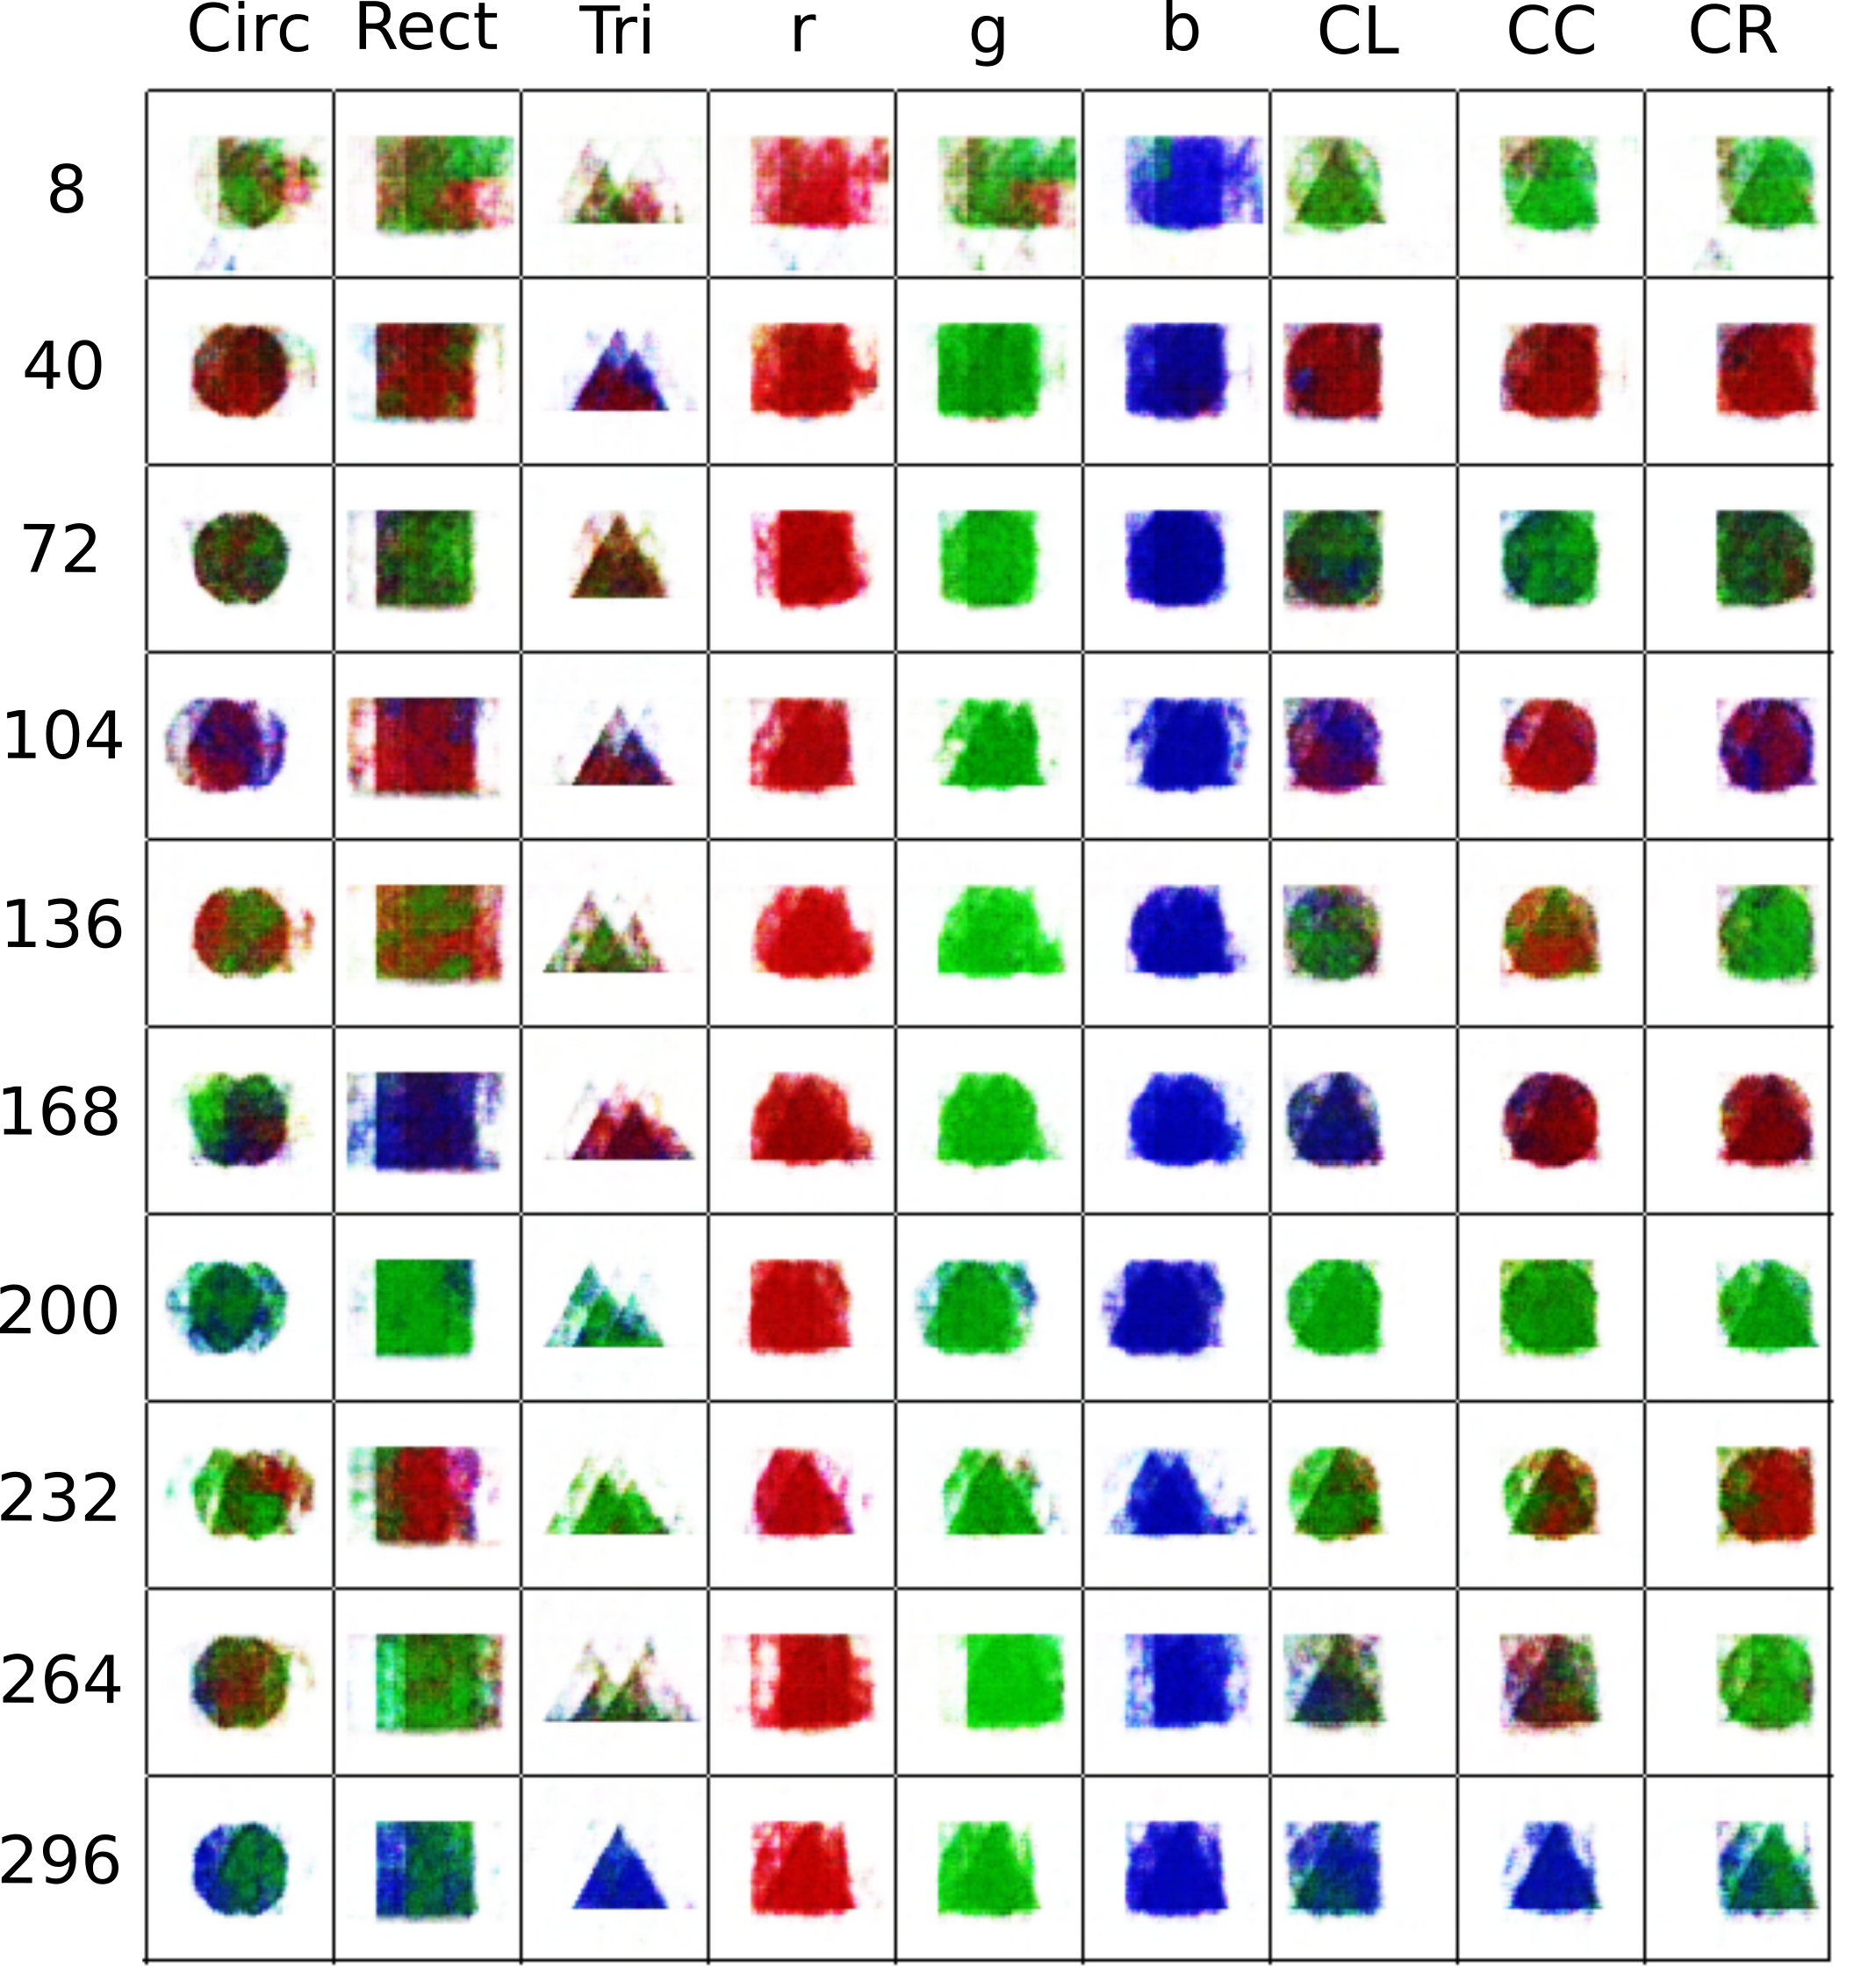
\includegraphics[width=0.75\textwidth]{Figs/shapes/singlelabel331A.png}
%\caption{Images generated of each word for different sizes of embedding using the MAE trained in experiment 1 run A.}
%\label{fig:331singleA}
%\end{figure}
%\begin{figure}
%\centering
%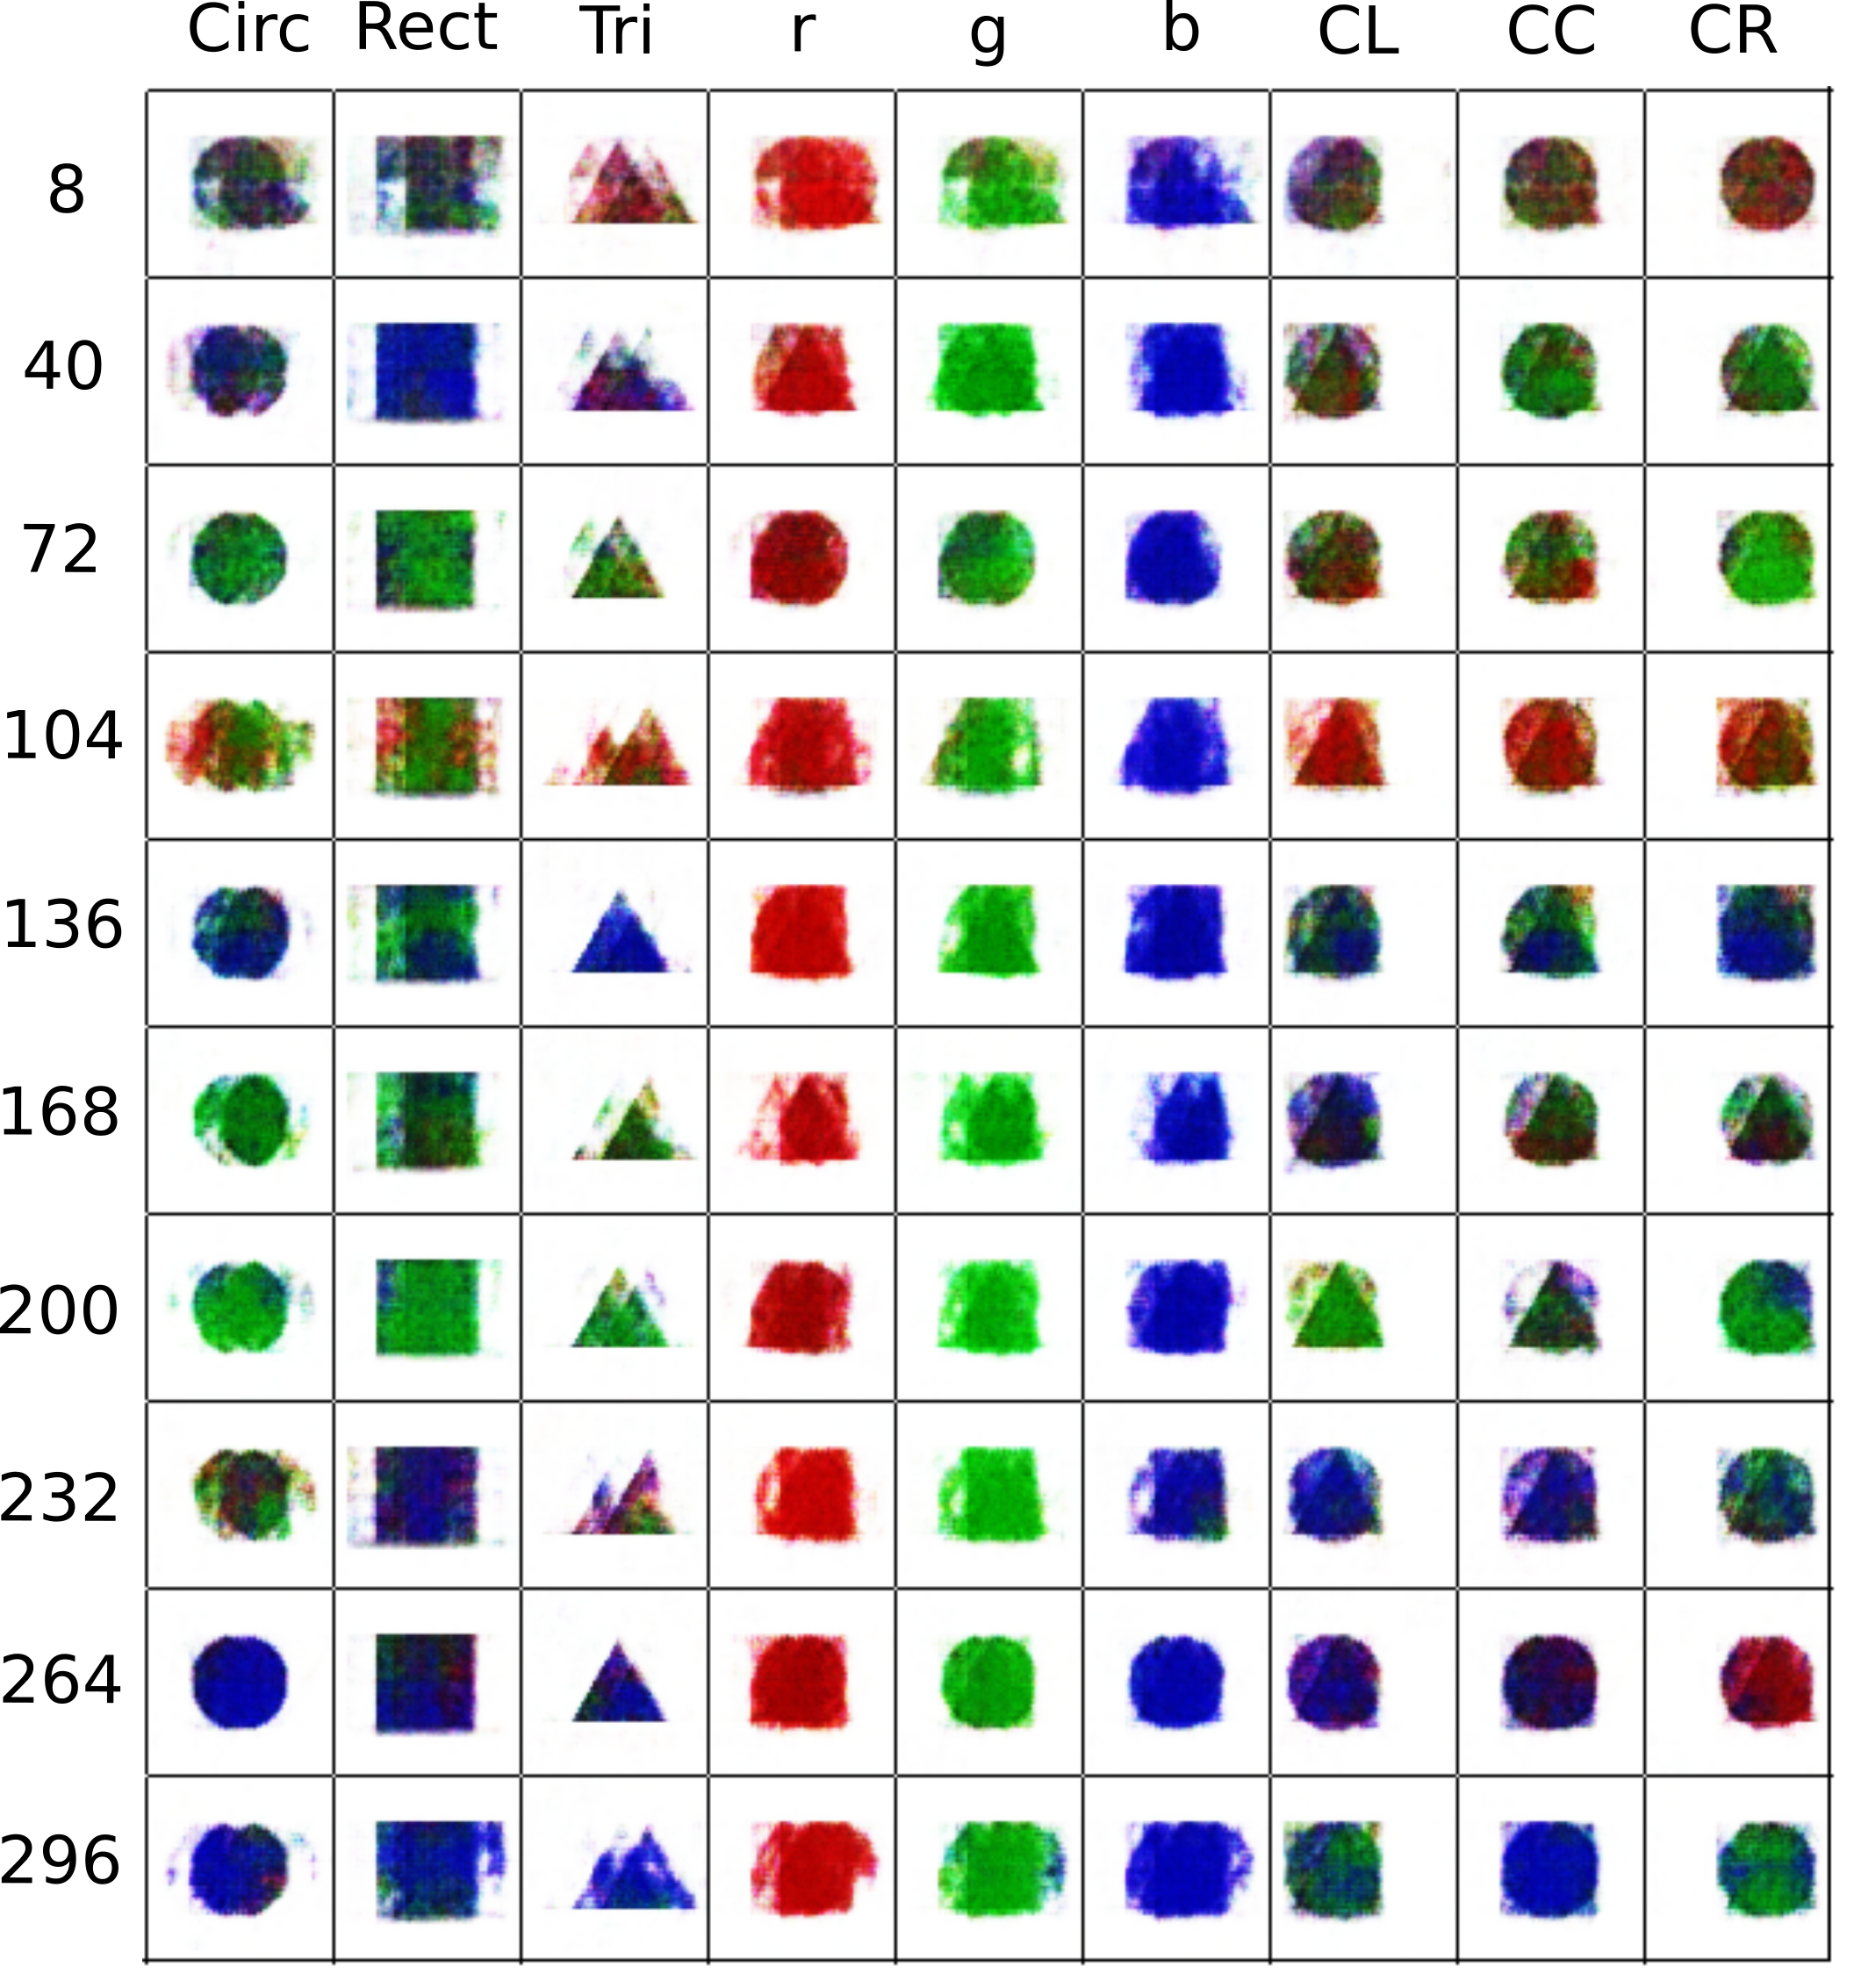
\includegraphics[width=0.75\textwidth]{Figs/shapes/singlelabel331B.png}
%\caption{Images generated of each word for different sizes of embedding using the MAE trained in experiment 1 run B.}
%\label{fig:331singleB}
%\end{figure}
%\begin{figure}
%\centering
%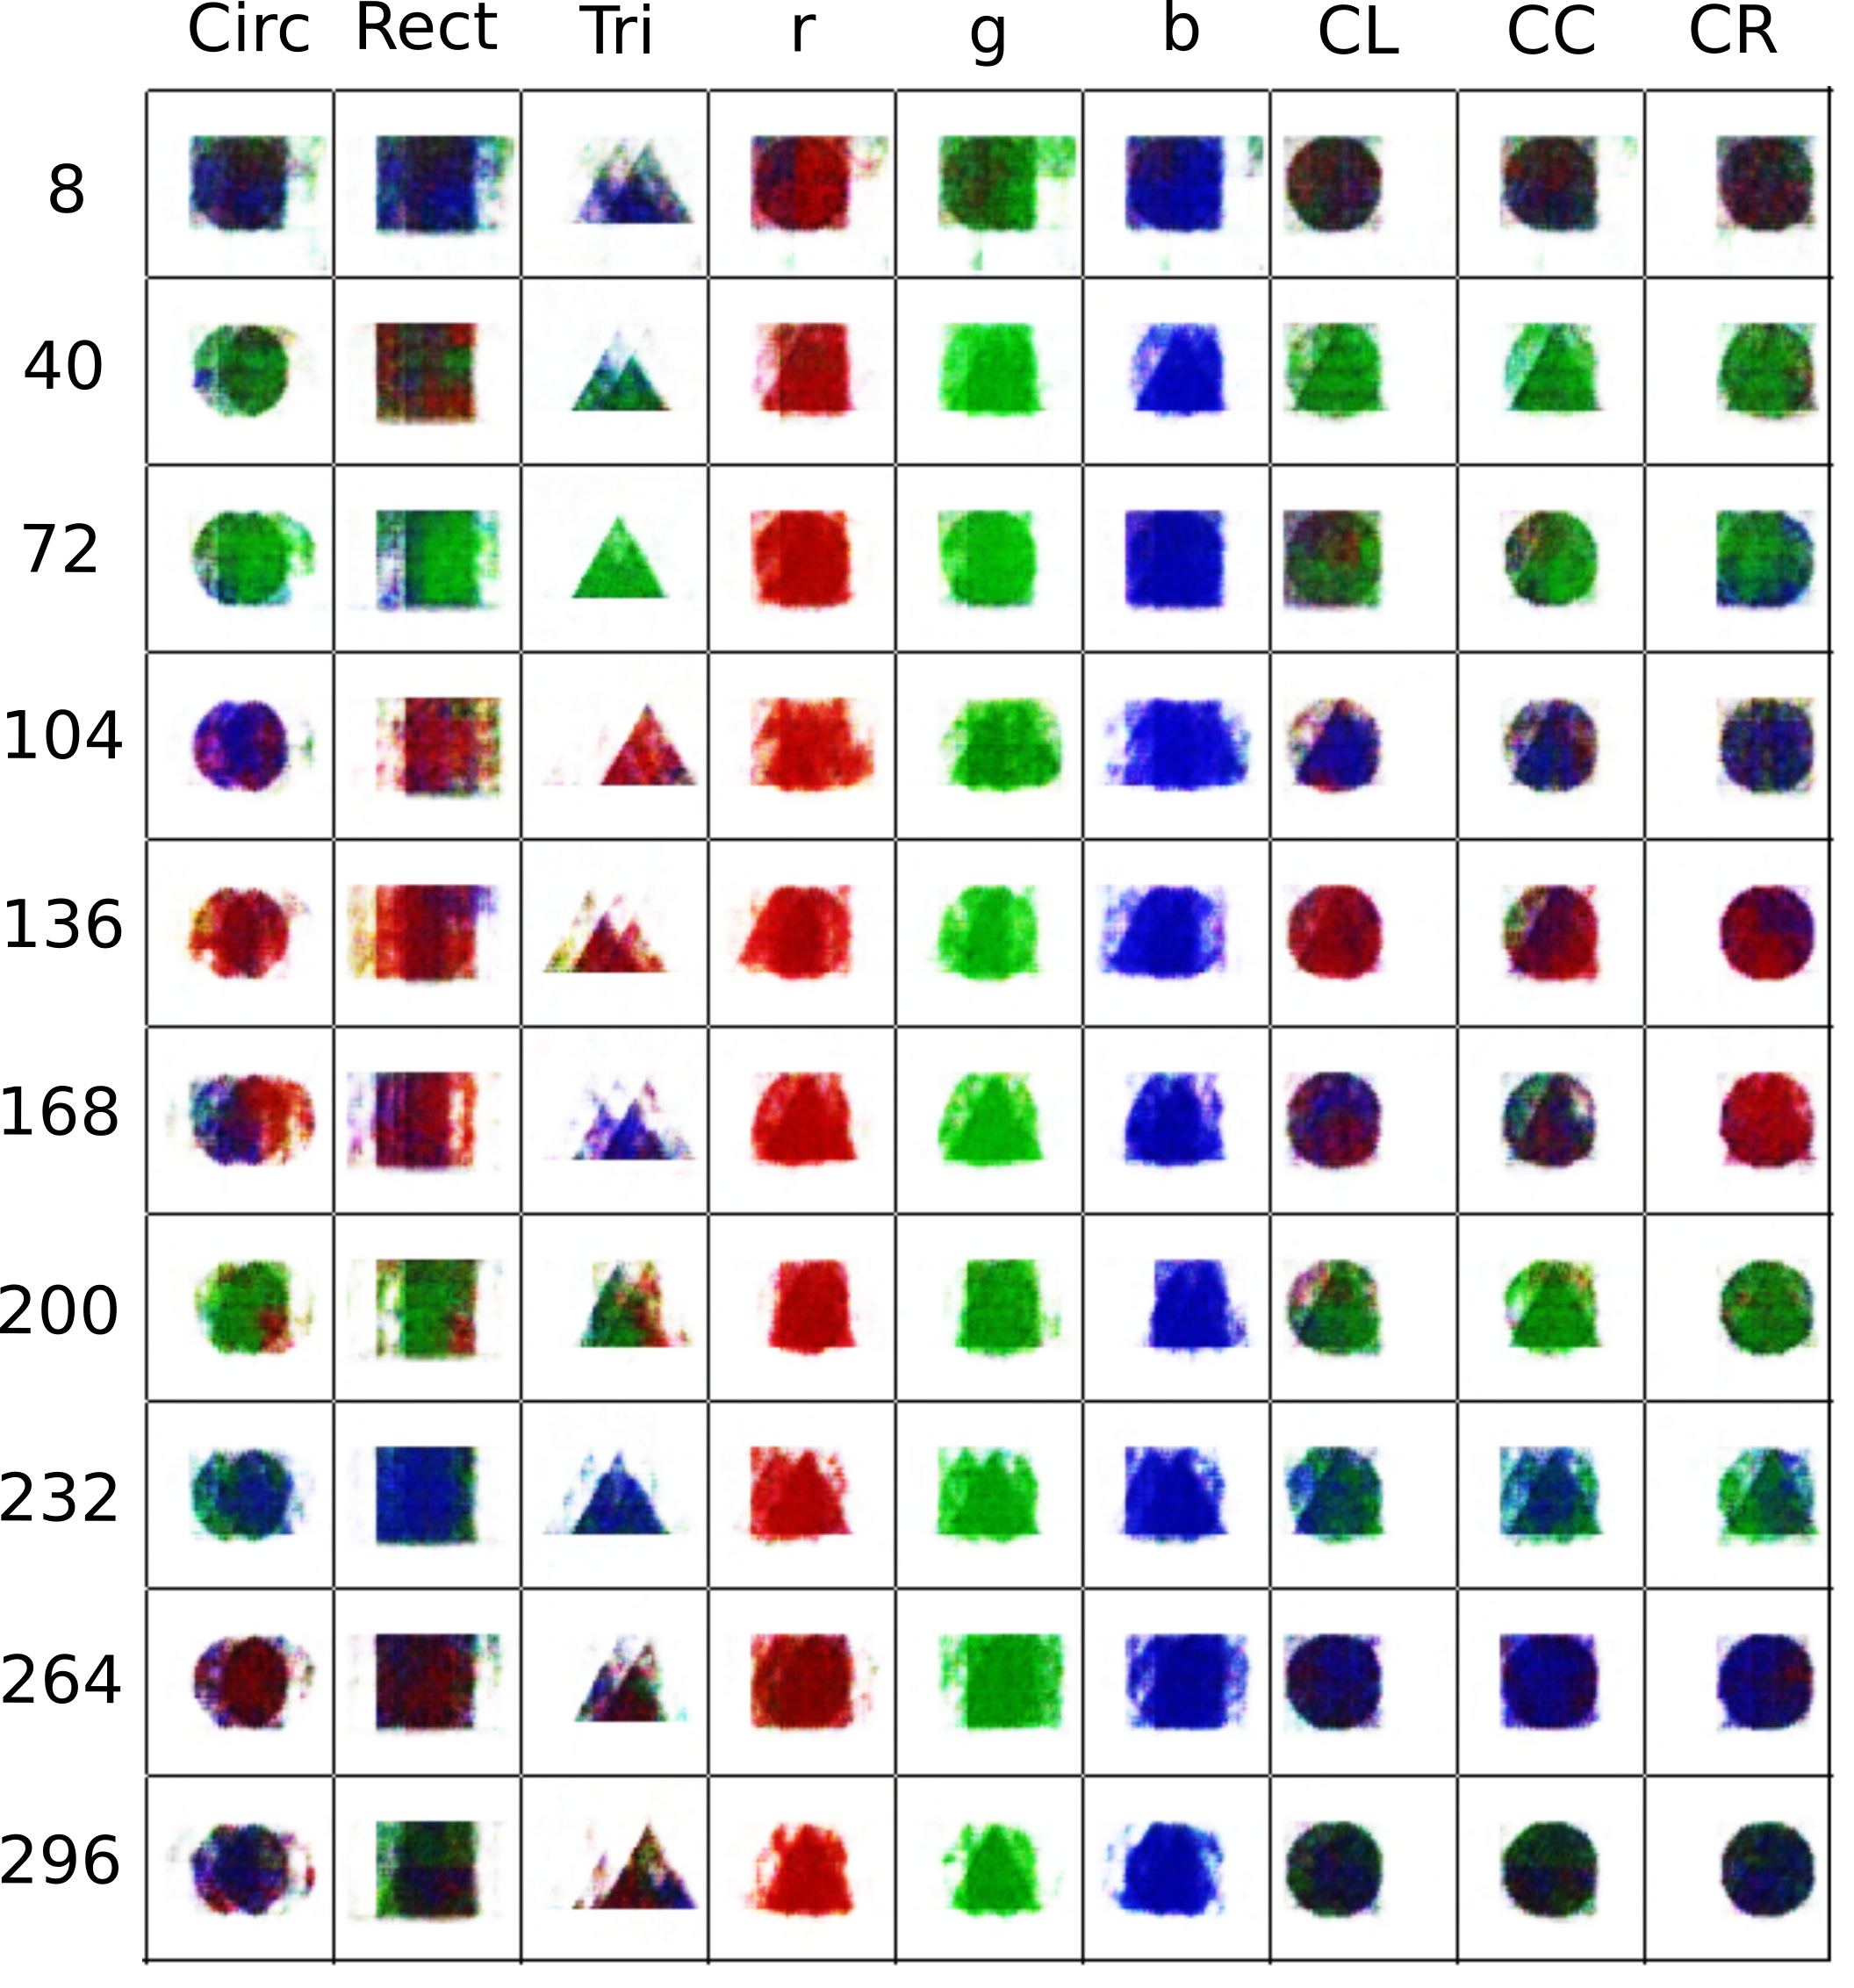
\includegraphics[width=0.75\textwidth]{Figs/shapes/singlelabel331C.png}
%\caption{Images generated of each word for different sizes of embedding using the MAE trained in experiment 1 run C.}
%\label{fig:331singleC}
%\end{figure}
%\begin{figure}
%\centering
%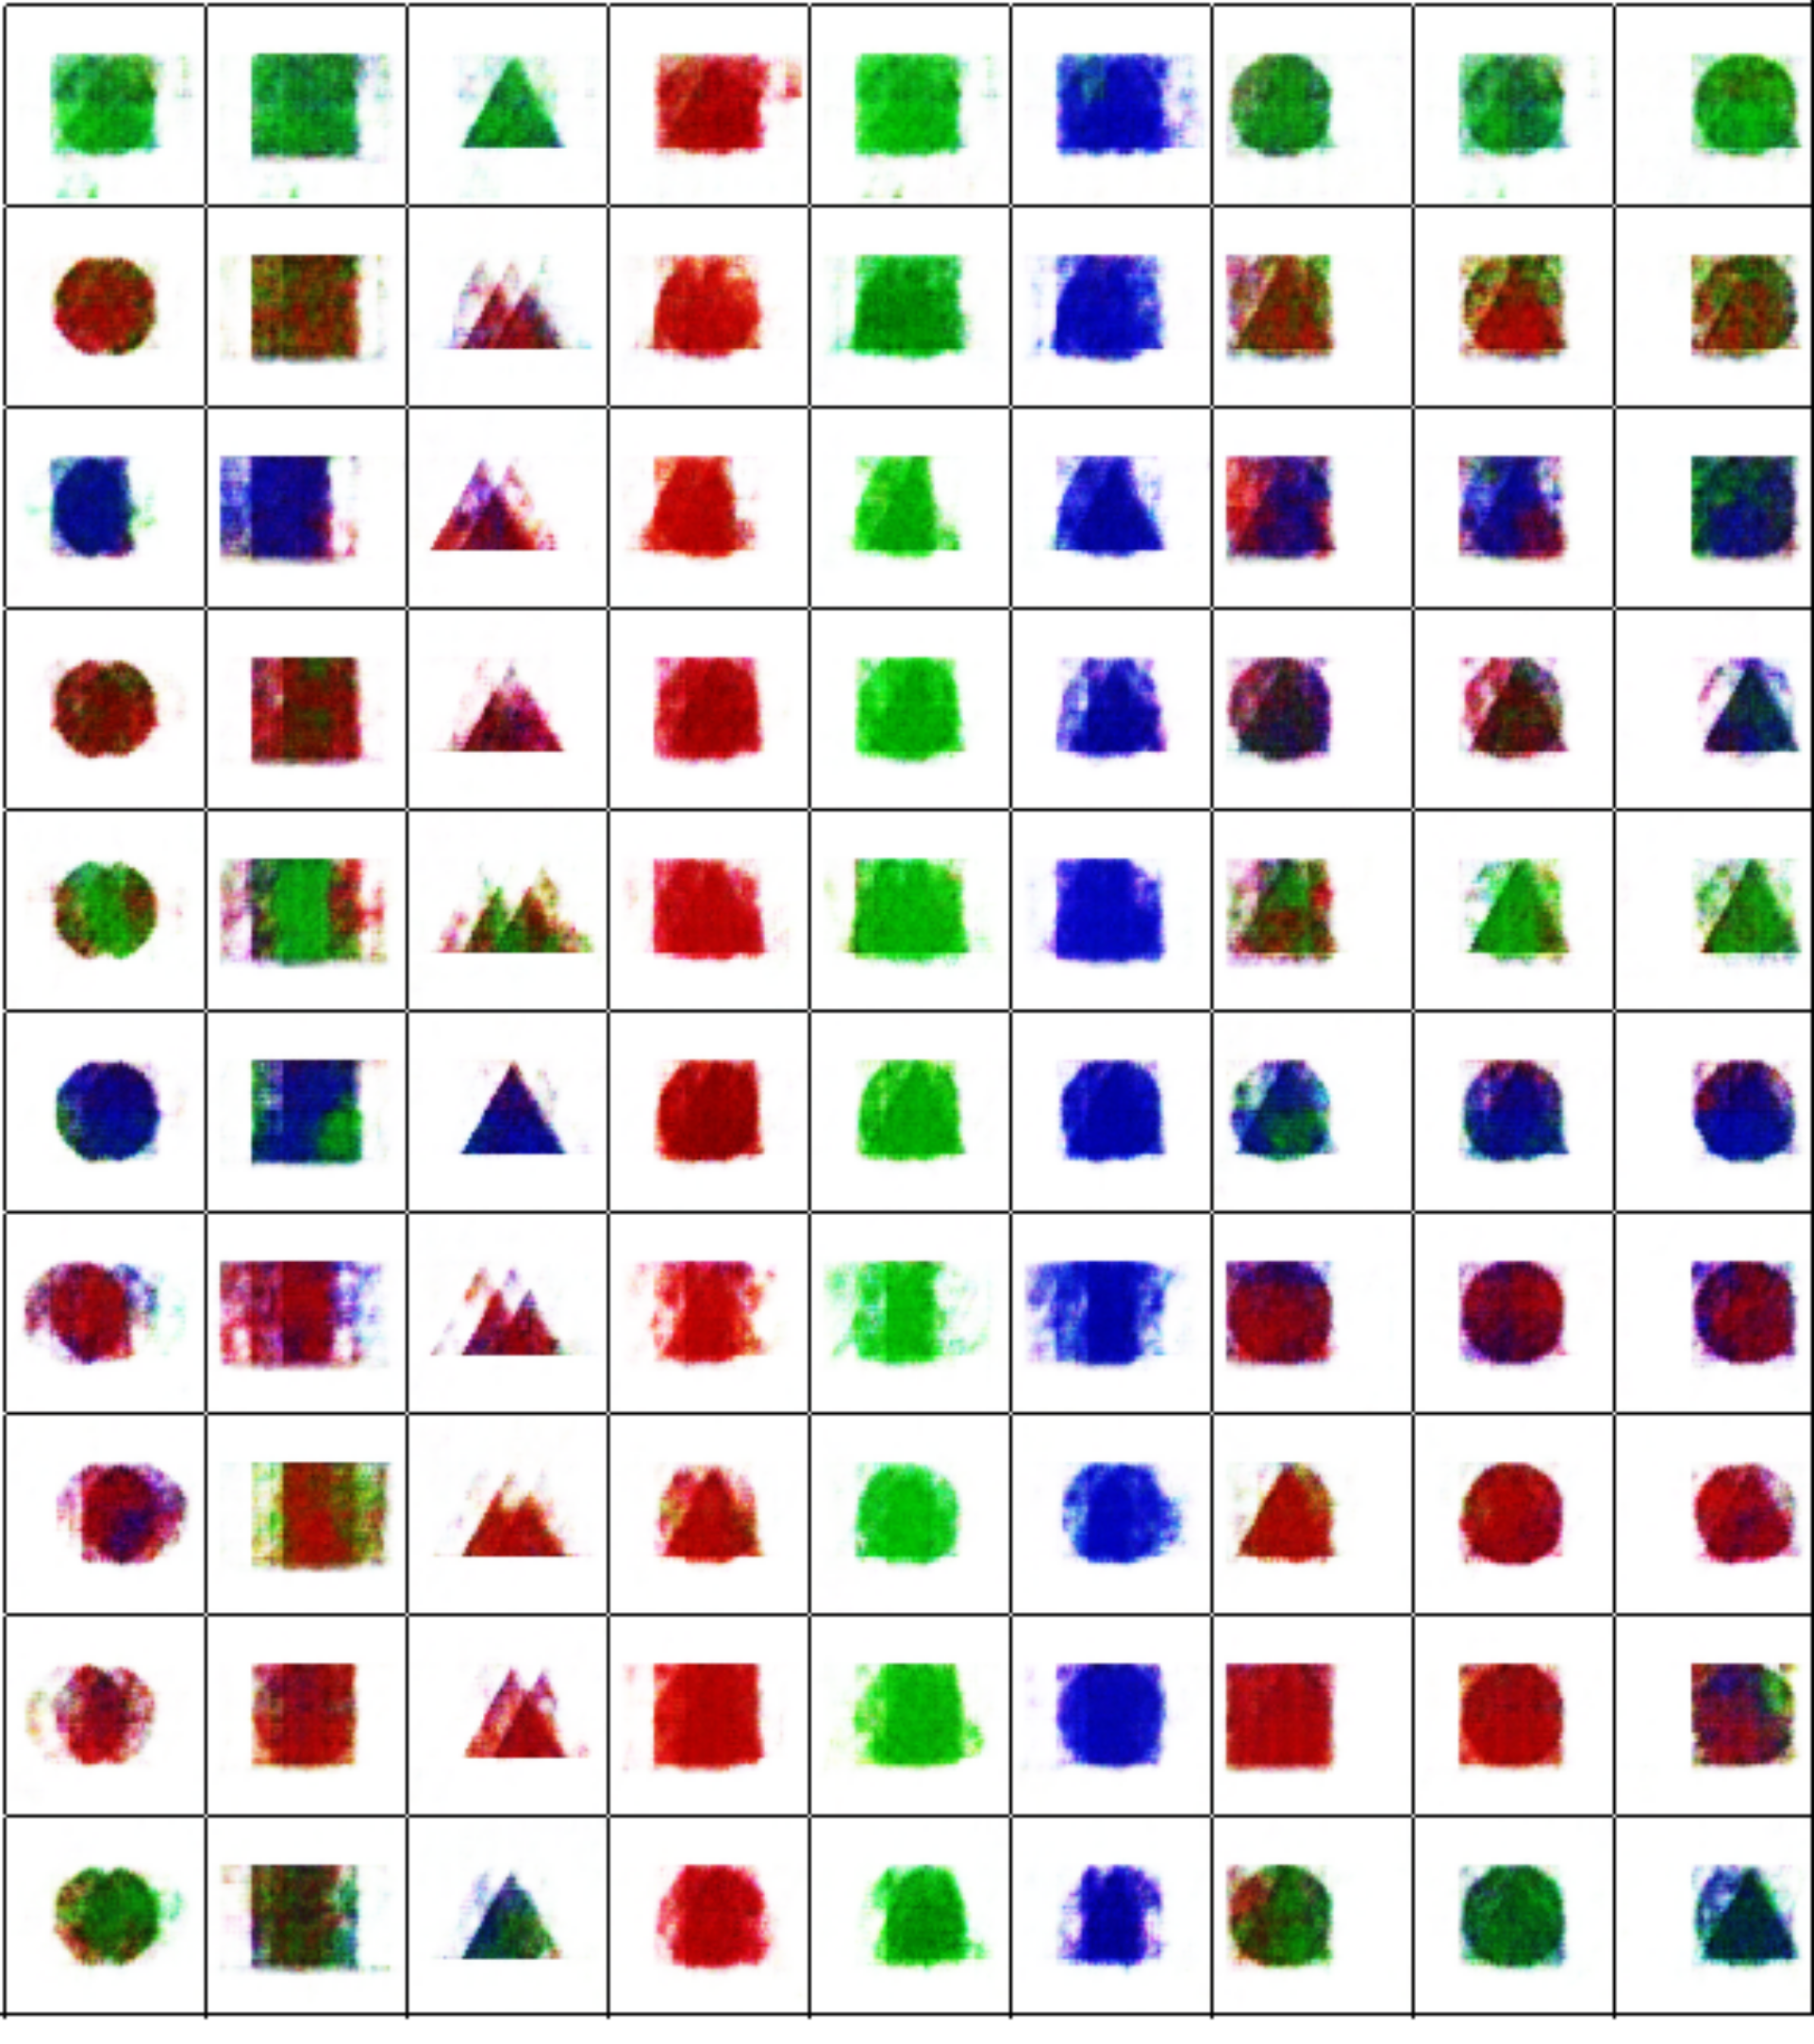
\includegraphics[width=0.75\textwidth]{Figs/shapes/singlelabel331D.png}
%\caption{Images generated of each word for different sizes of embedding using the MAE trained in experiment 1 run D.}
%\label{fig:331singleD}
%\end{figure}



The number of weight updates during training is given by \autoref{eqn:updates}.

\begin{equation}\label{eqn:updates}
u = E \times S \times Obj \times C \times Sz \times pos
\end{equation}

Where $u$ is th number of updates, $E$ the number of epochs of training, $S$ the number of samples for each shape, colour, size, position combination, $Obj$ the number of shapes, $C$ the number of colours, $Sz$ the number of sizes and $pos$ the number of positions.


\begin{table}
\centering
\begin{tabular}{|c|c|c|c|c|c|c|c|}
\hline
Experiment & Samples & Shapes & Colours & Sizes & Positions & Updates per Epoch \\ \hline
Exp 1 & 50 & 3 & 3 & 1 & 3 & 1350 \\ \hline
Exp 2 & 50 & 3 & 3 & 3 & 3 & 4050 \\ \hline
Exp 3 & 50 & 3 & 3 & 3 & 9 & 12150 \\ \hline
Exp 4 & 50 & 3 & 7 & 3 & 9 & 28350 \\ \hline

\end{tabular}
\caption{Number of weight updates per Epoch for each experiment.}
\label{tab:updatesperEpoch}
\end{table}

\autoref{tab:updatesperEpoch} shows how many times per epoch the weights of the MAE are updated in each experiment. As more data is available in later experiments due to the increase in number of shape-colour-size-position combinations, there are more weight updates per epoch. 

The total number of weight updates a MAE recieves therefore depends on the data it is trained on. Whilst all MAEs in experiment 3 are trained for a total of 100 epochs, for the MAEs which are pretrained, 50 of these epochs are with less data than the full amount available in experiment 3.


%\begin{figure}
%\centering
%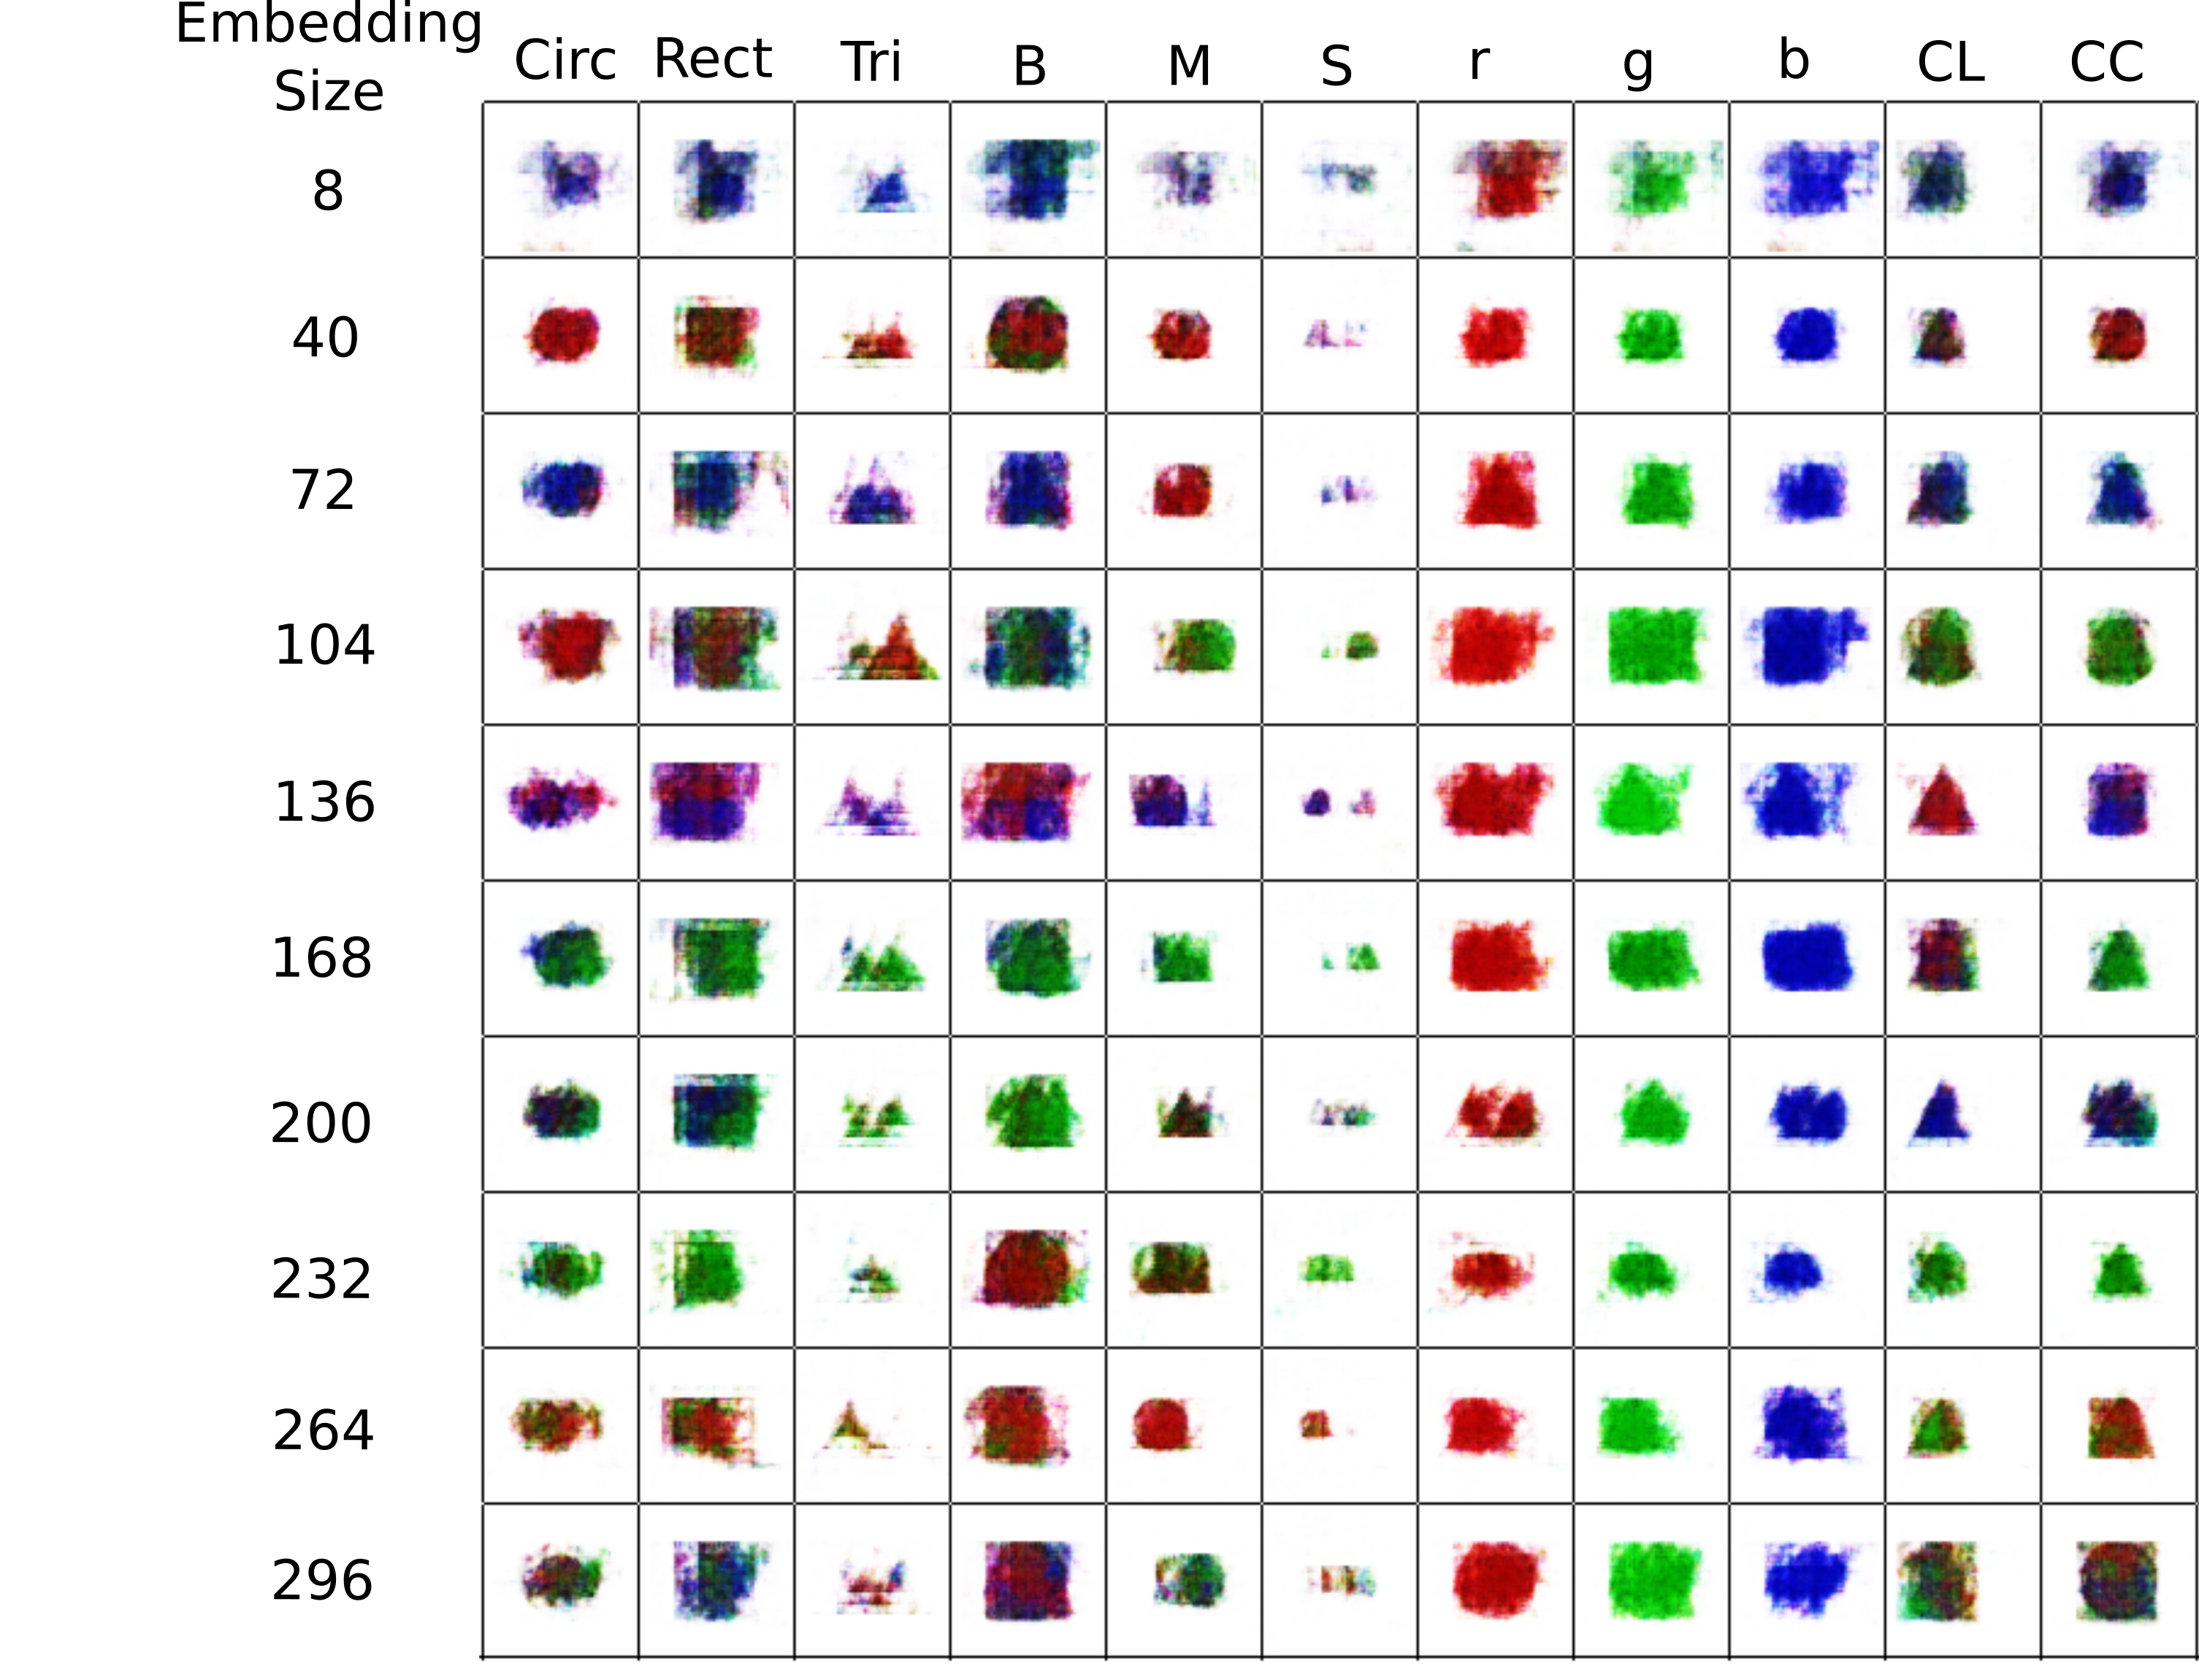
\includegraphics[width=0.75\textwidth]{Figs/shapes/singlelabel333A.png}
%\caption{Images generated of each word for different sizes of embedding using the MAE trained in experiment 2 run A.}
%\label{fig:333singleA}
%\end{figure}
%\begin{figure}
%\centering
%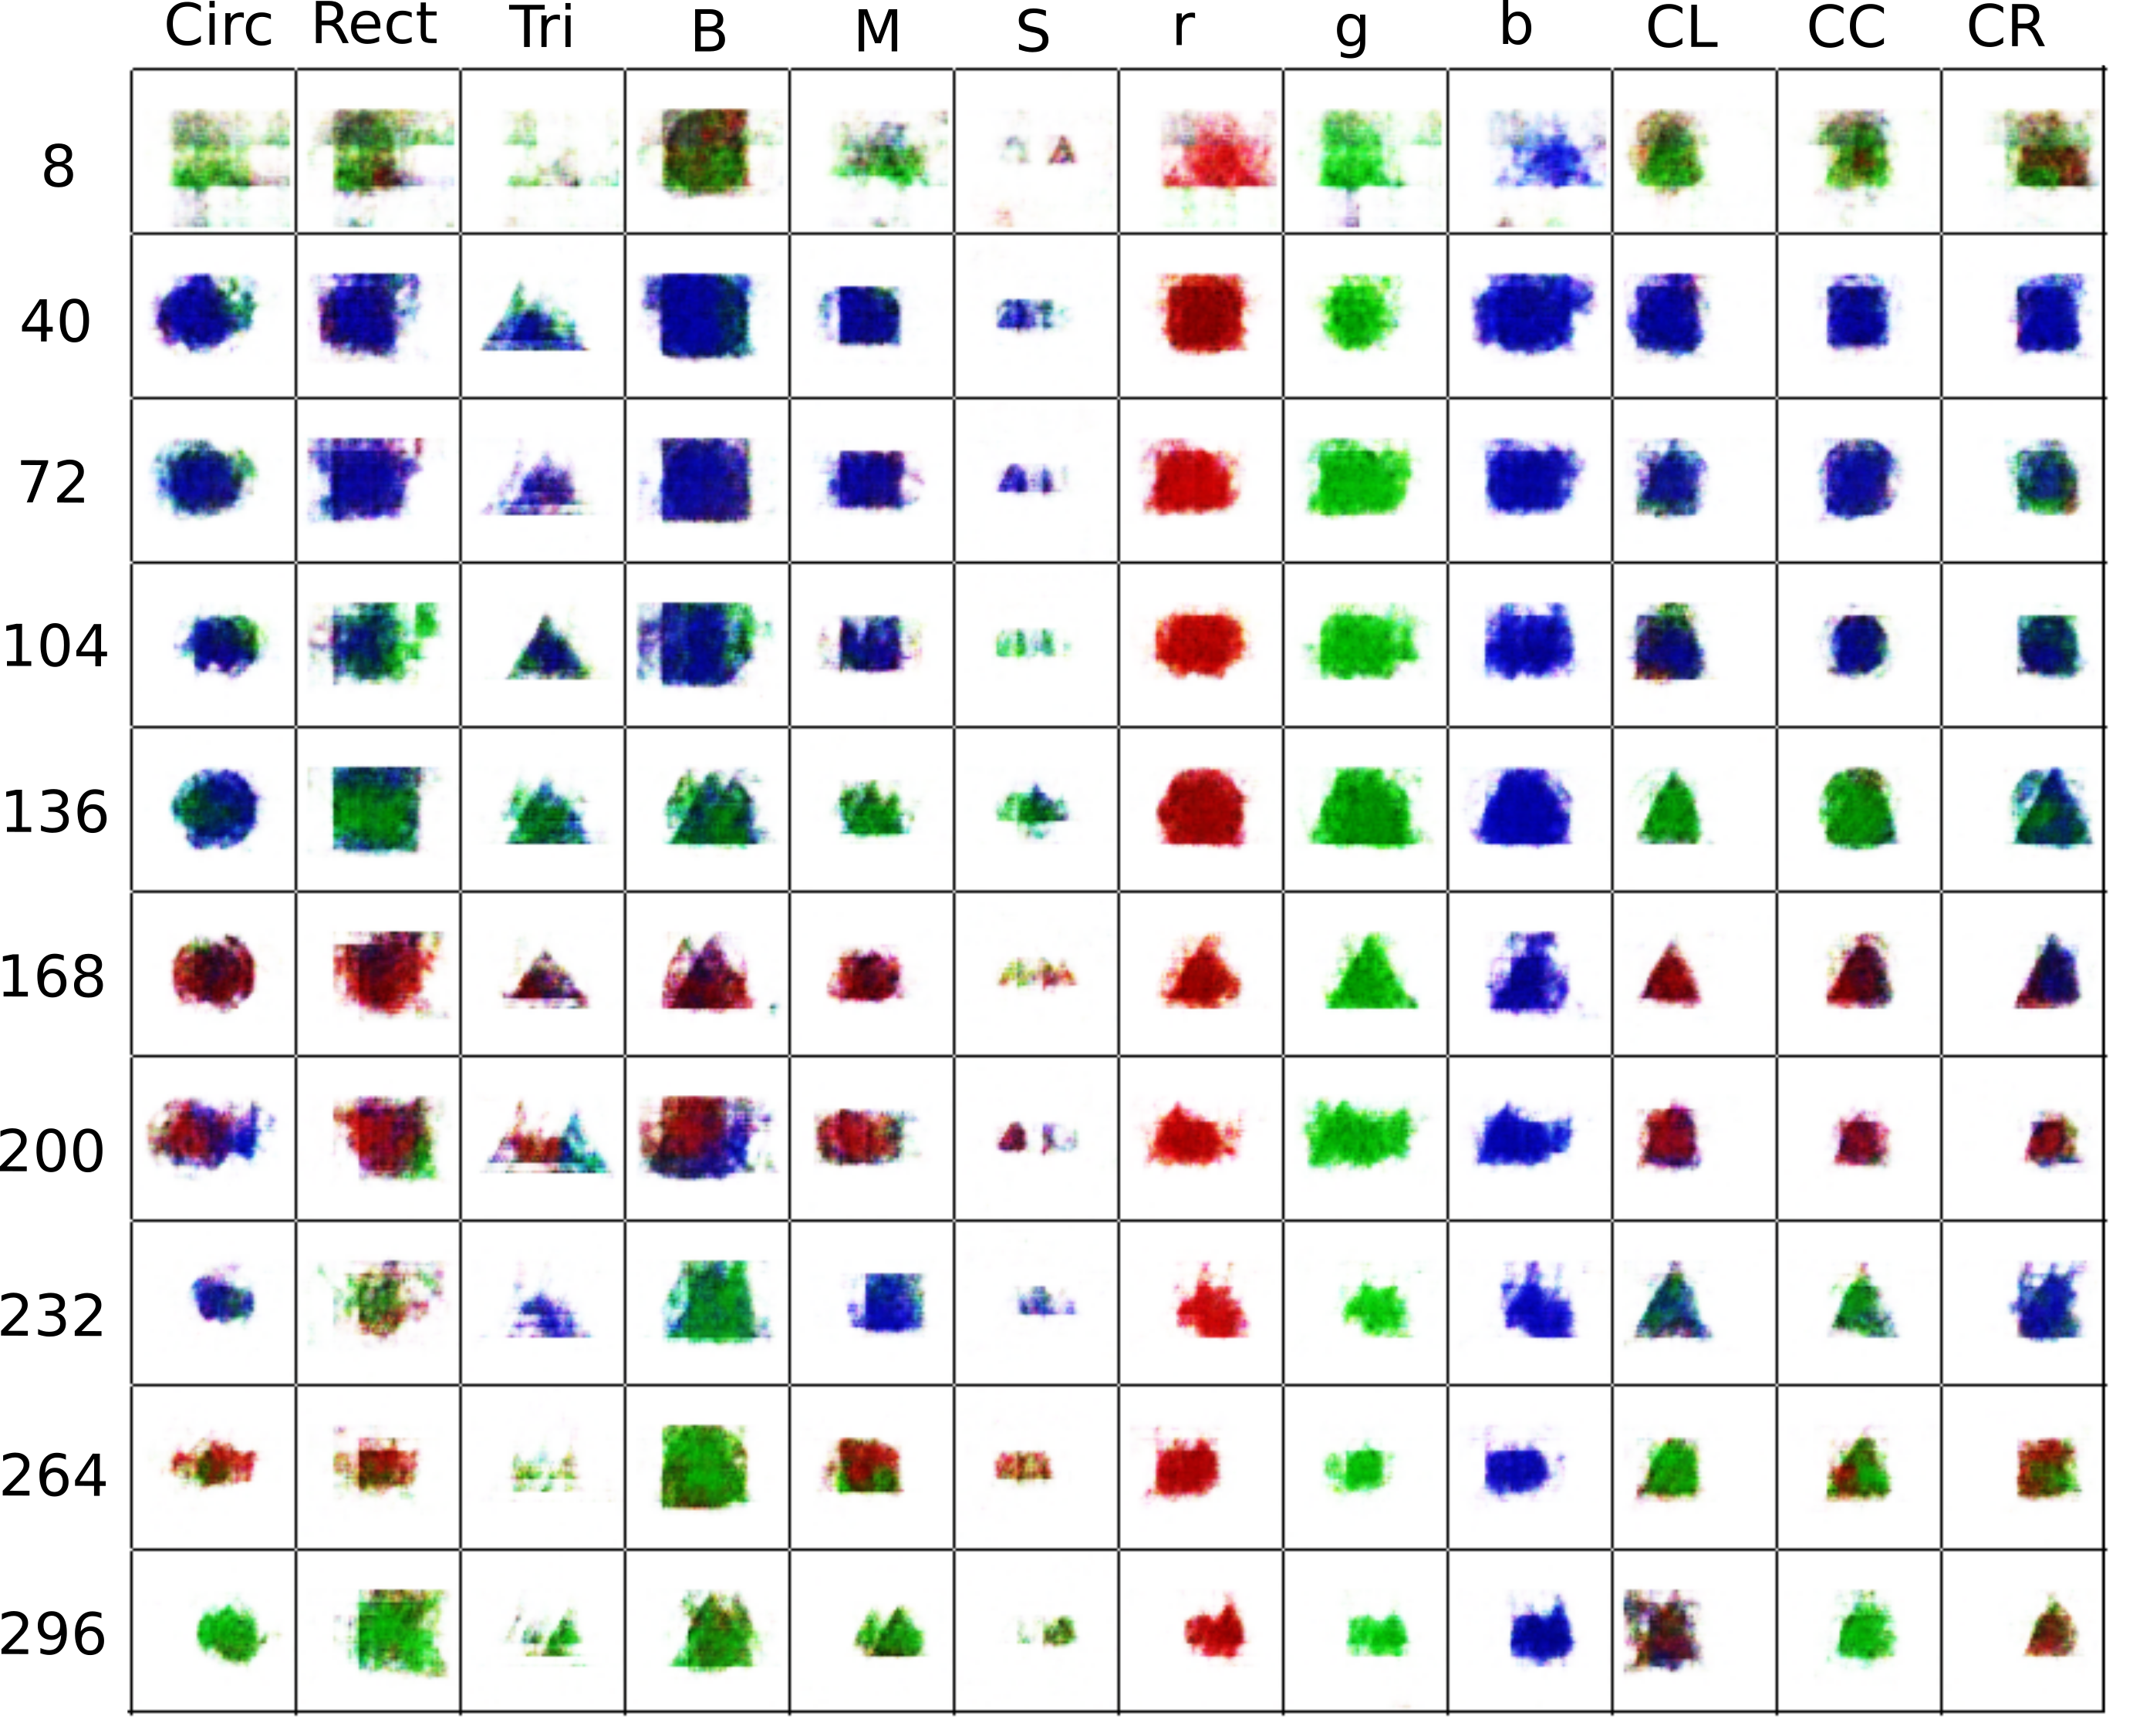
\includegraphics[width=0.75\textwidth]{Figs/shapes/singlelabel333B.png}
%\caption{Images generated of each word for different sizes of embedding using the MAE trained in experiment 2 run B.}
%\label{fig:333singleB}
%\end{figure}
%\begin{figure}
%\centering
%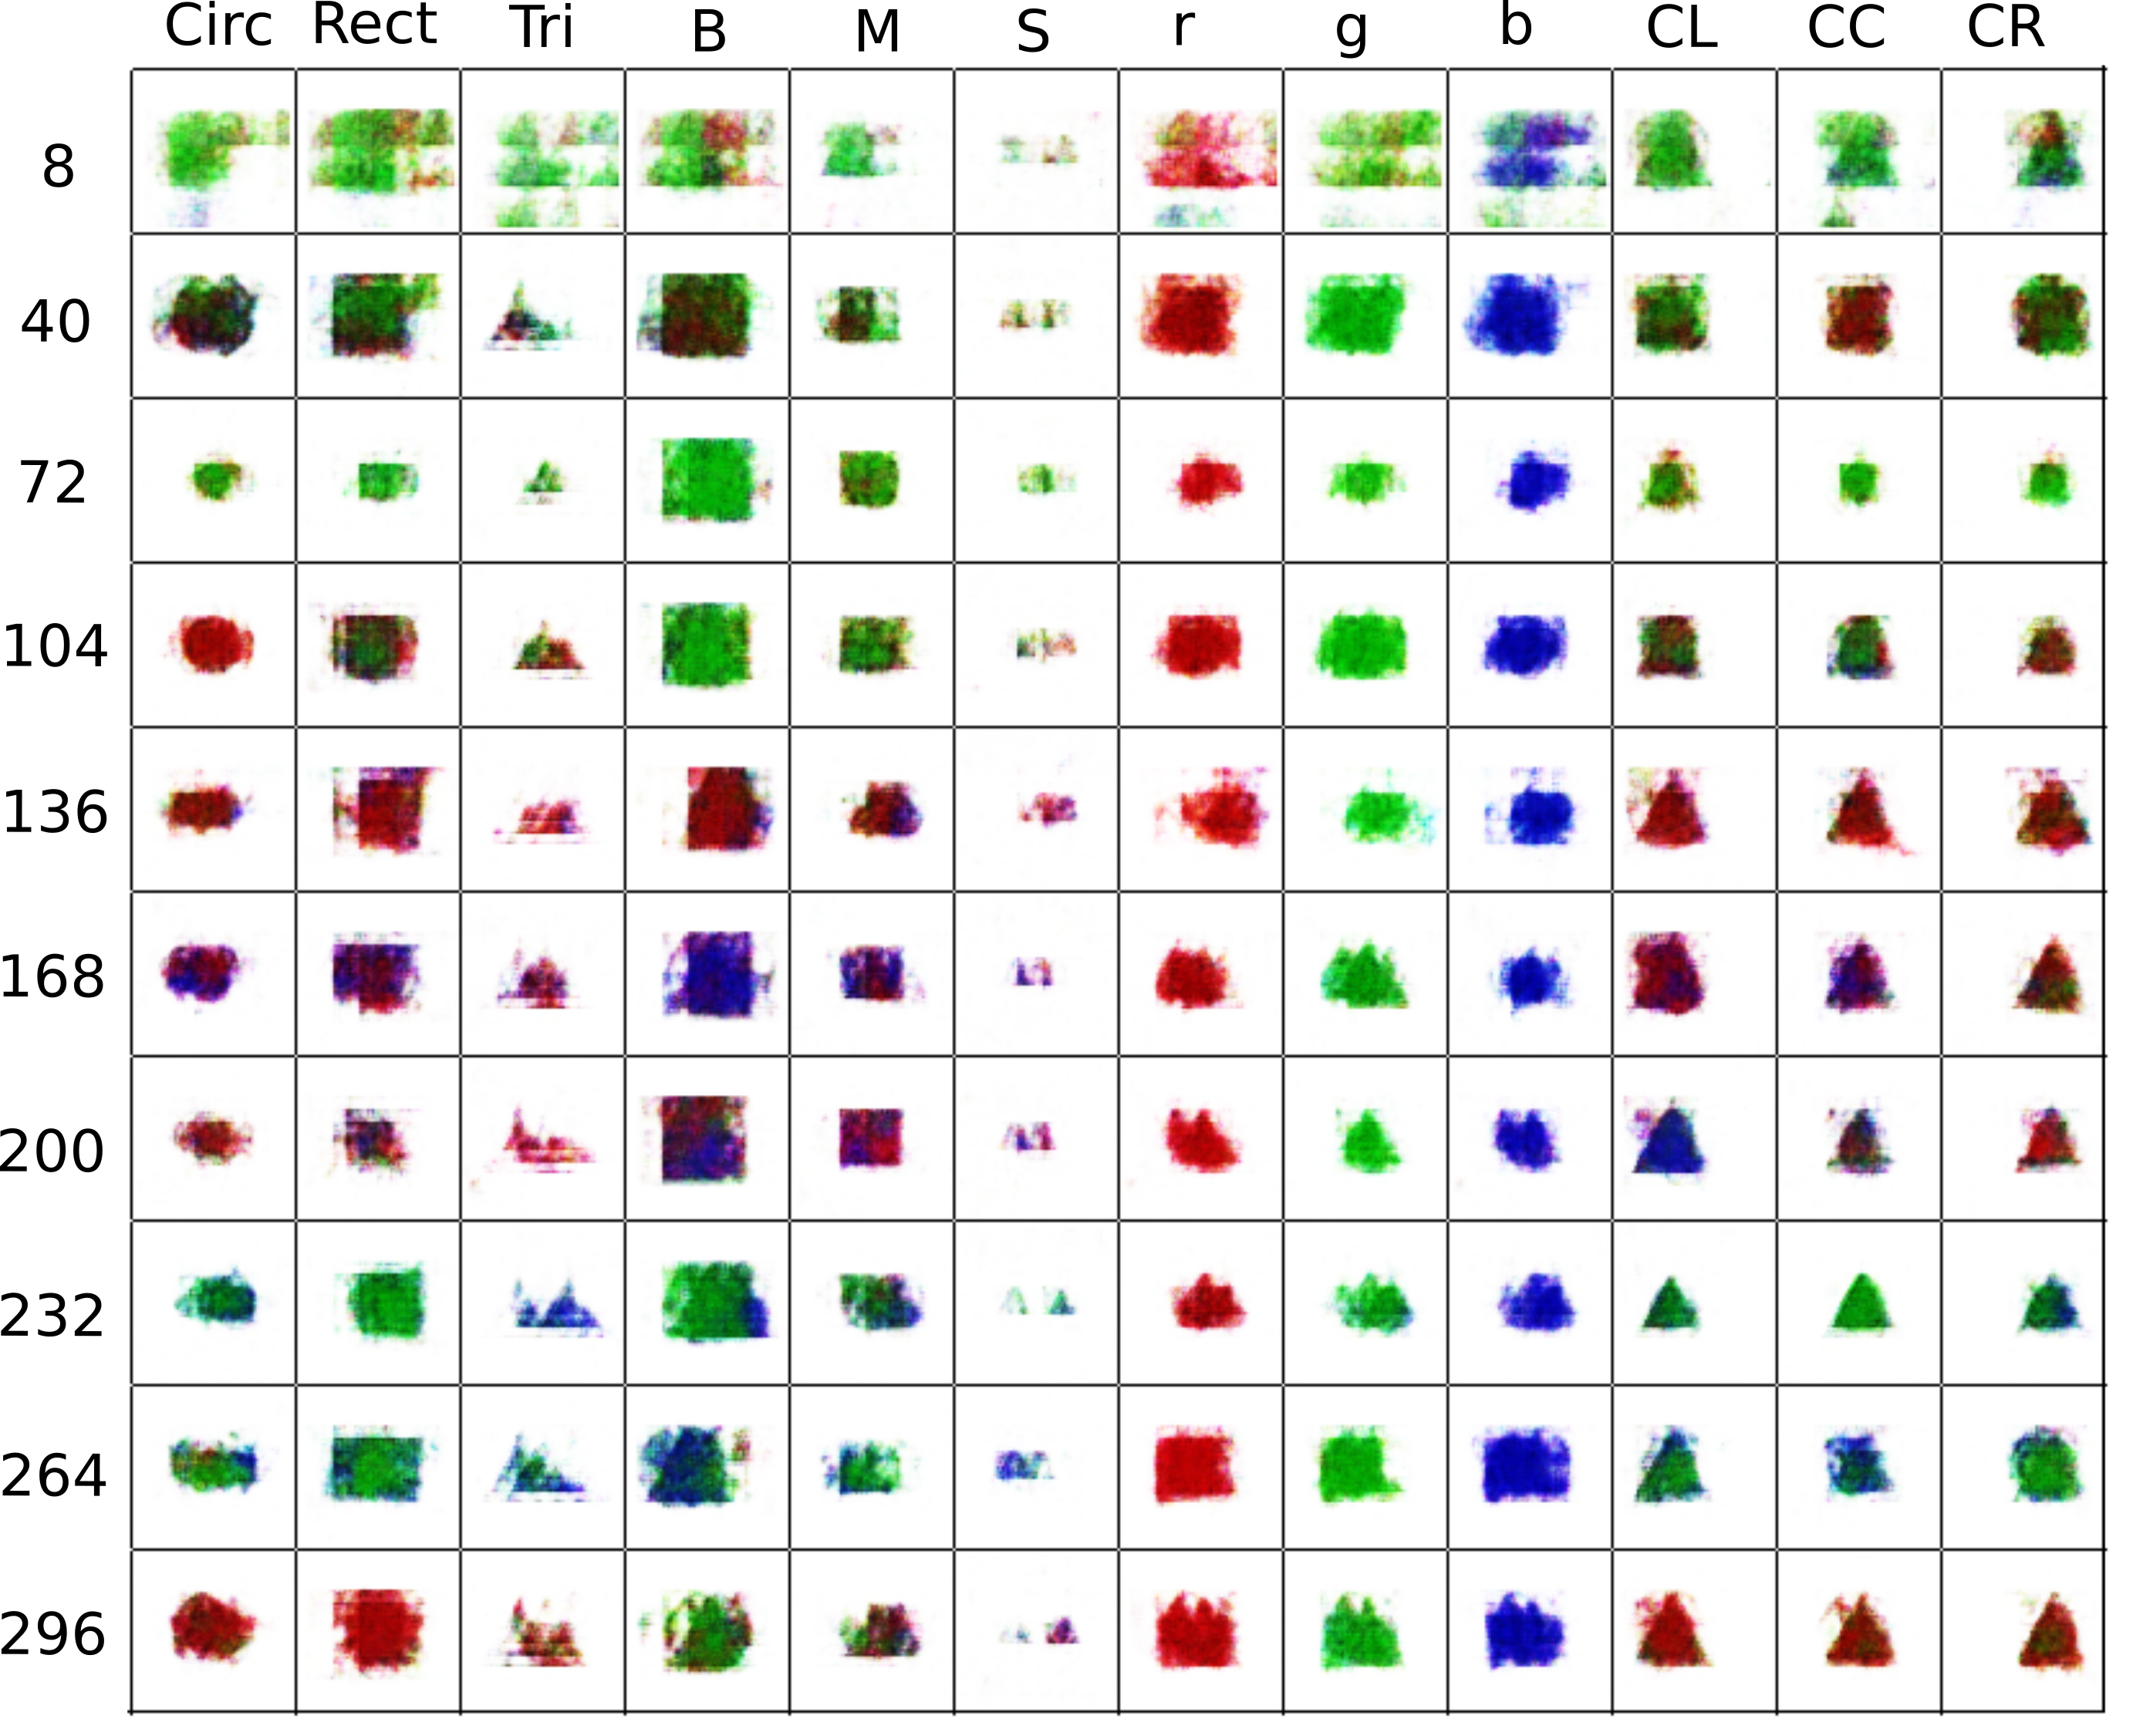
\includegraphics[width=0.75\textwidth]{Figs/shapes/singlelabel333C.png}
%\caption{Images generated of each word for different sizes of embedding using the MAE trained in experiment 2 run C.}
%\label{fig:333singleC}
%\end{figure}
%\begin{figure}
%\centering
%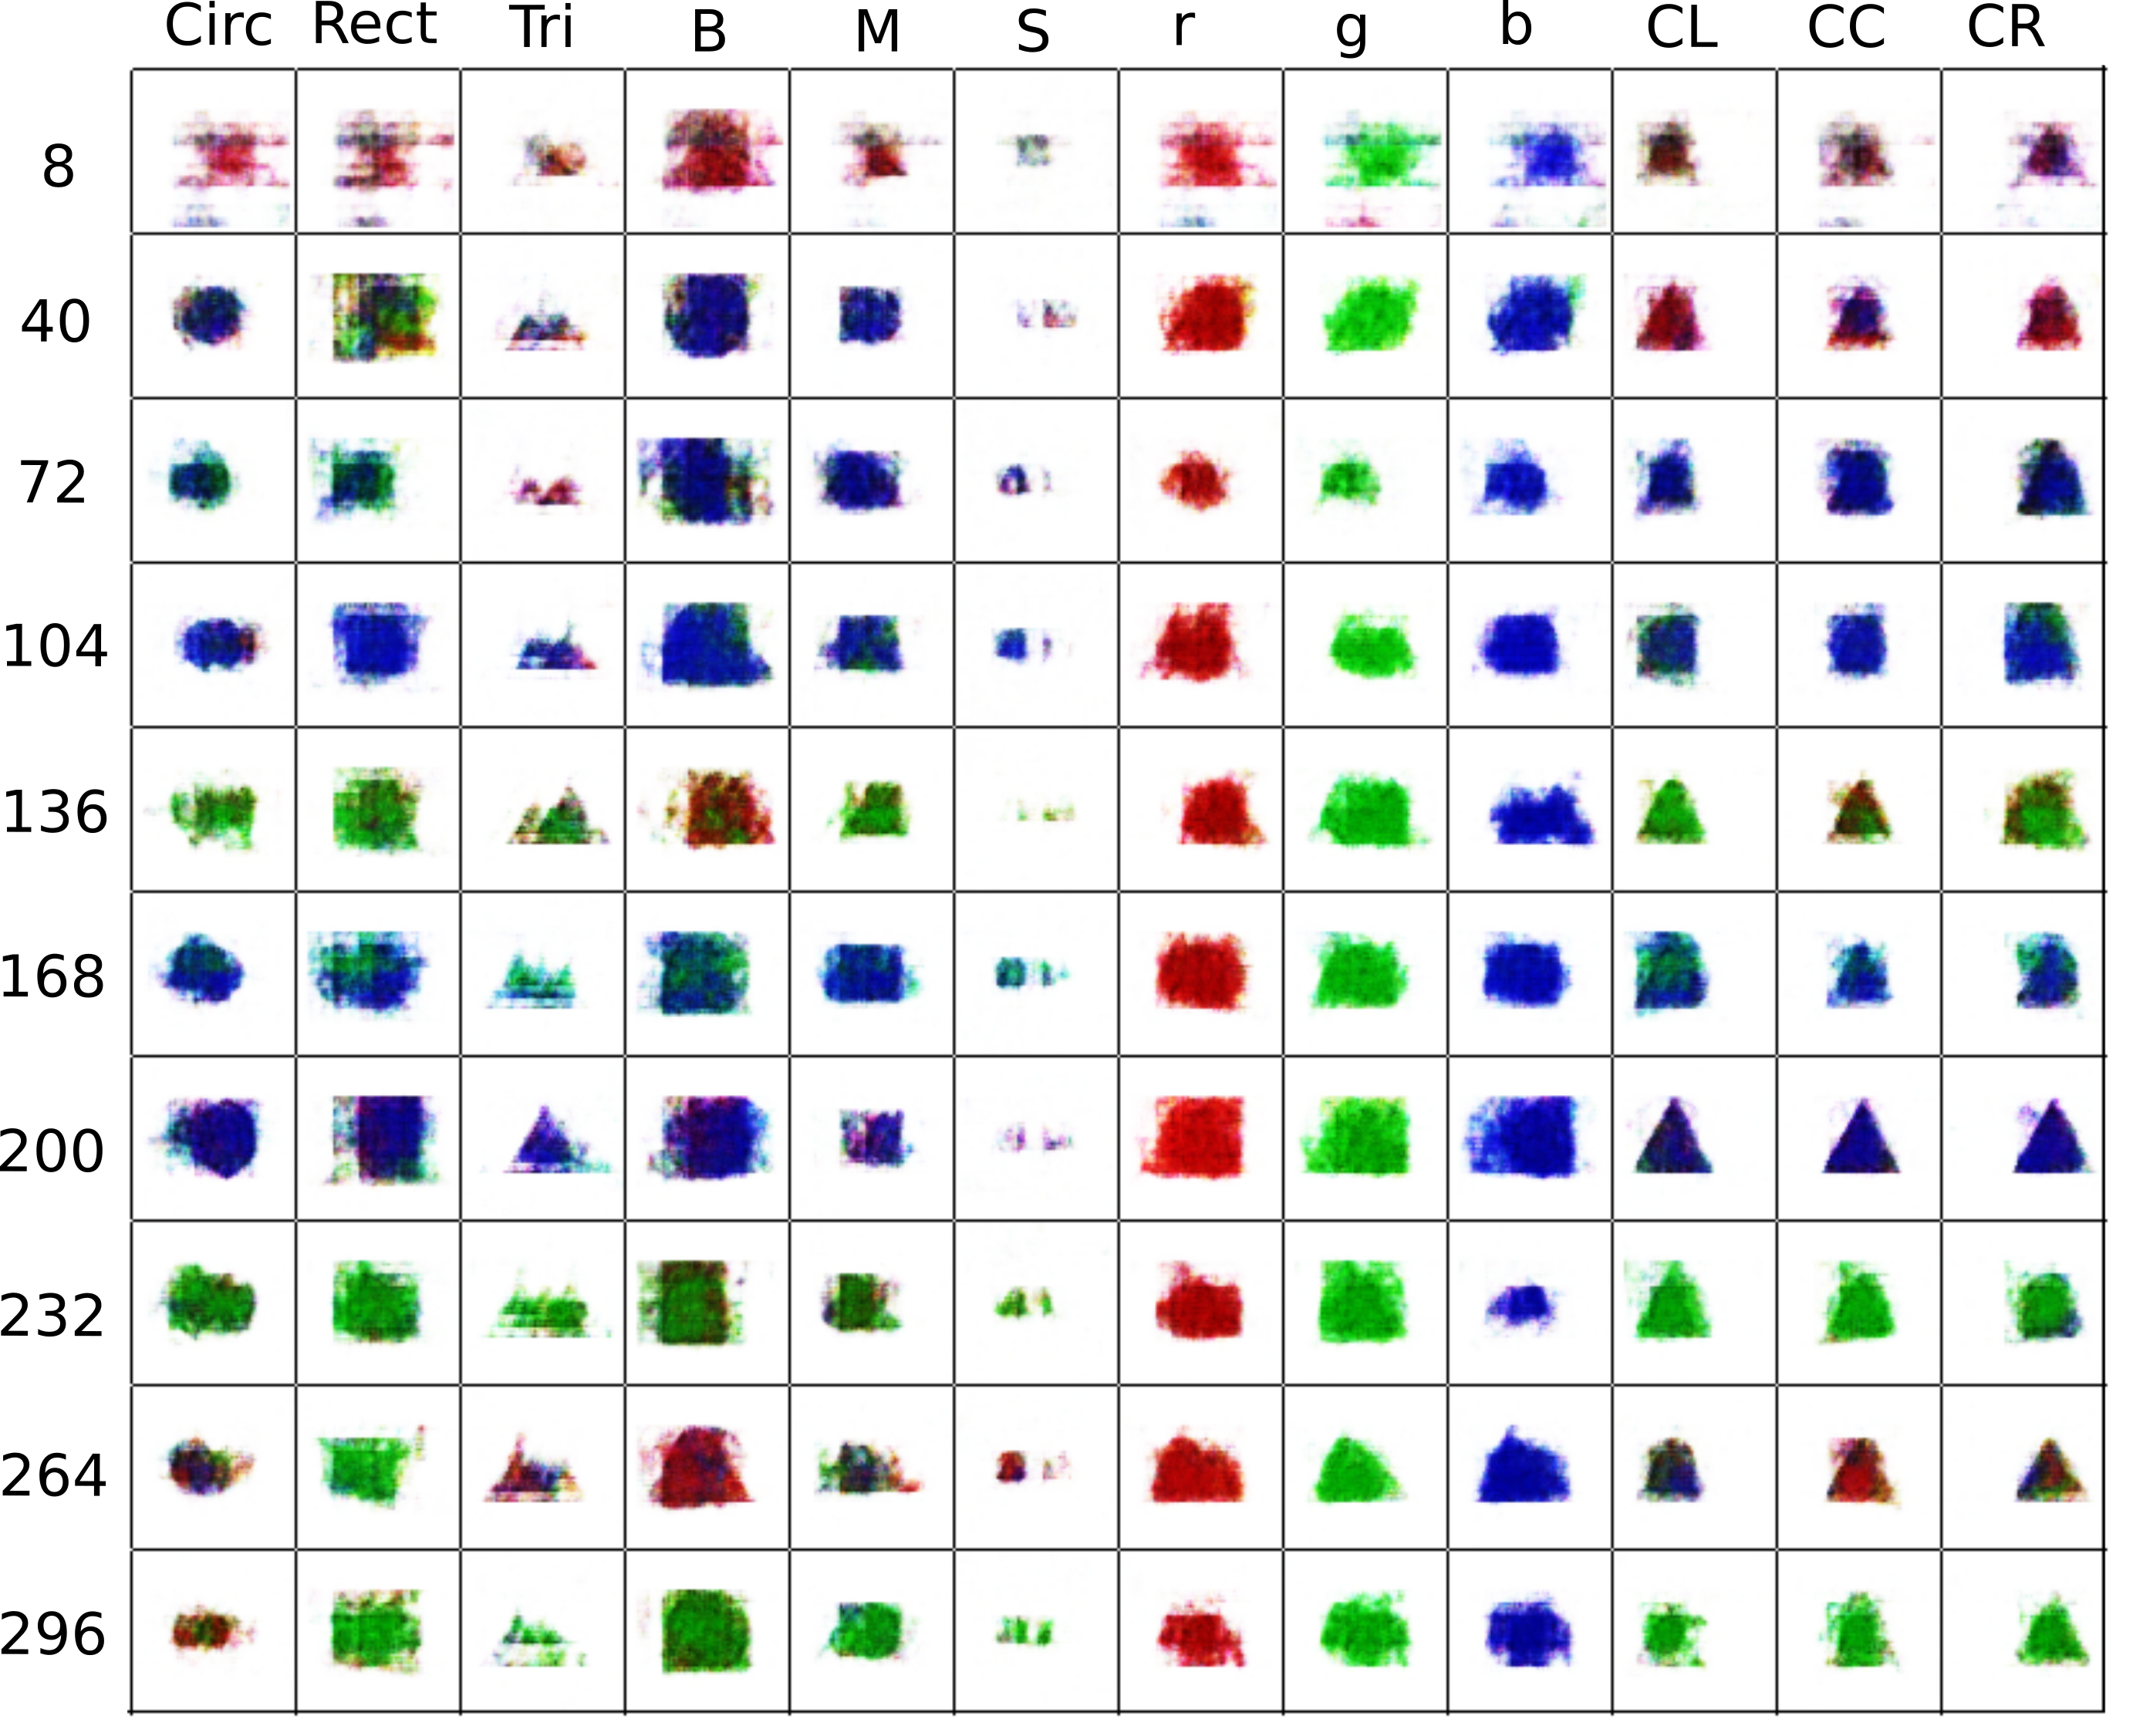
\includegraphics[width=0.75\textwidth]{Figs/shapes/singlelabel333D.png}
%\caption{Images generated of each word for different sizes of embedding using the MAE trained in experiment 2 run D.}
%\label{fig:333singleD}
%\end{figure}
%
%\begin{figure}
%\centering
%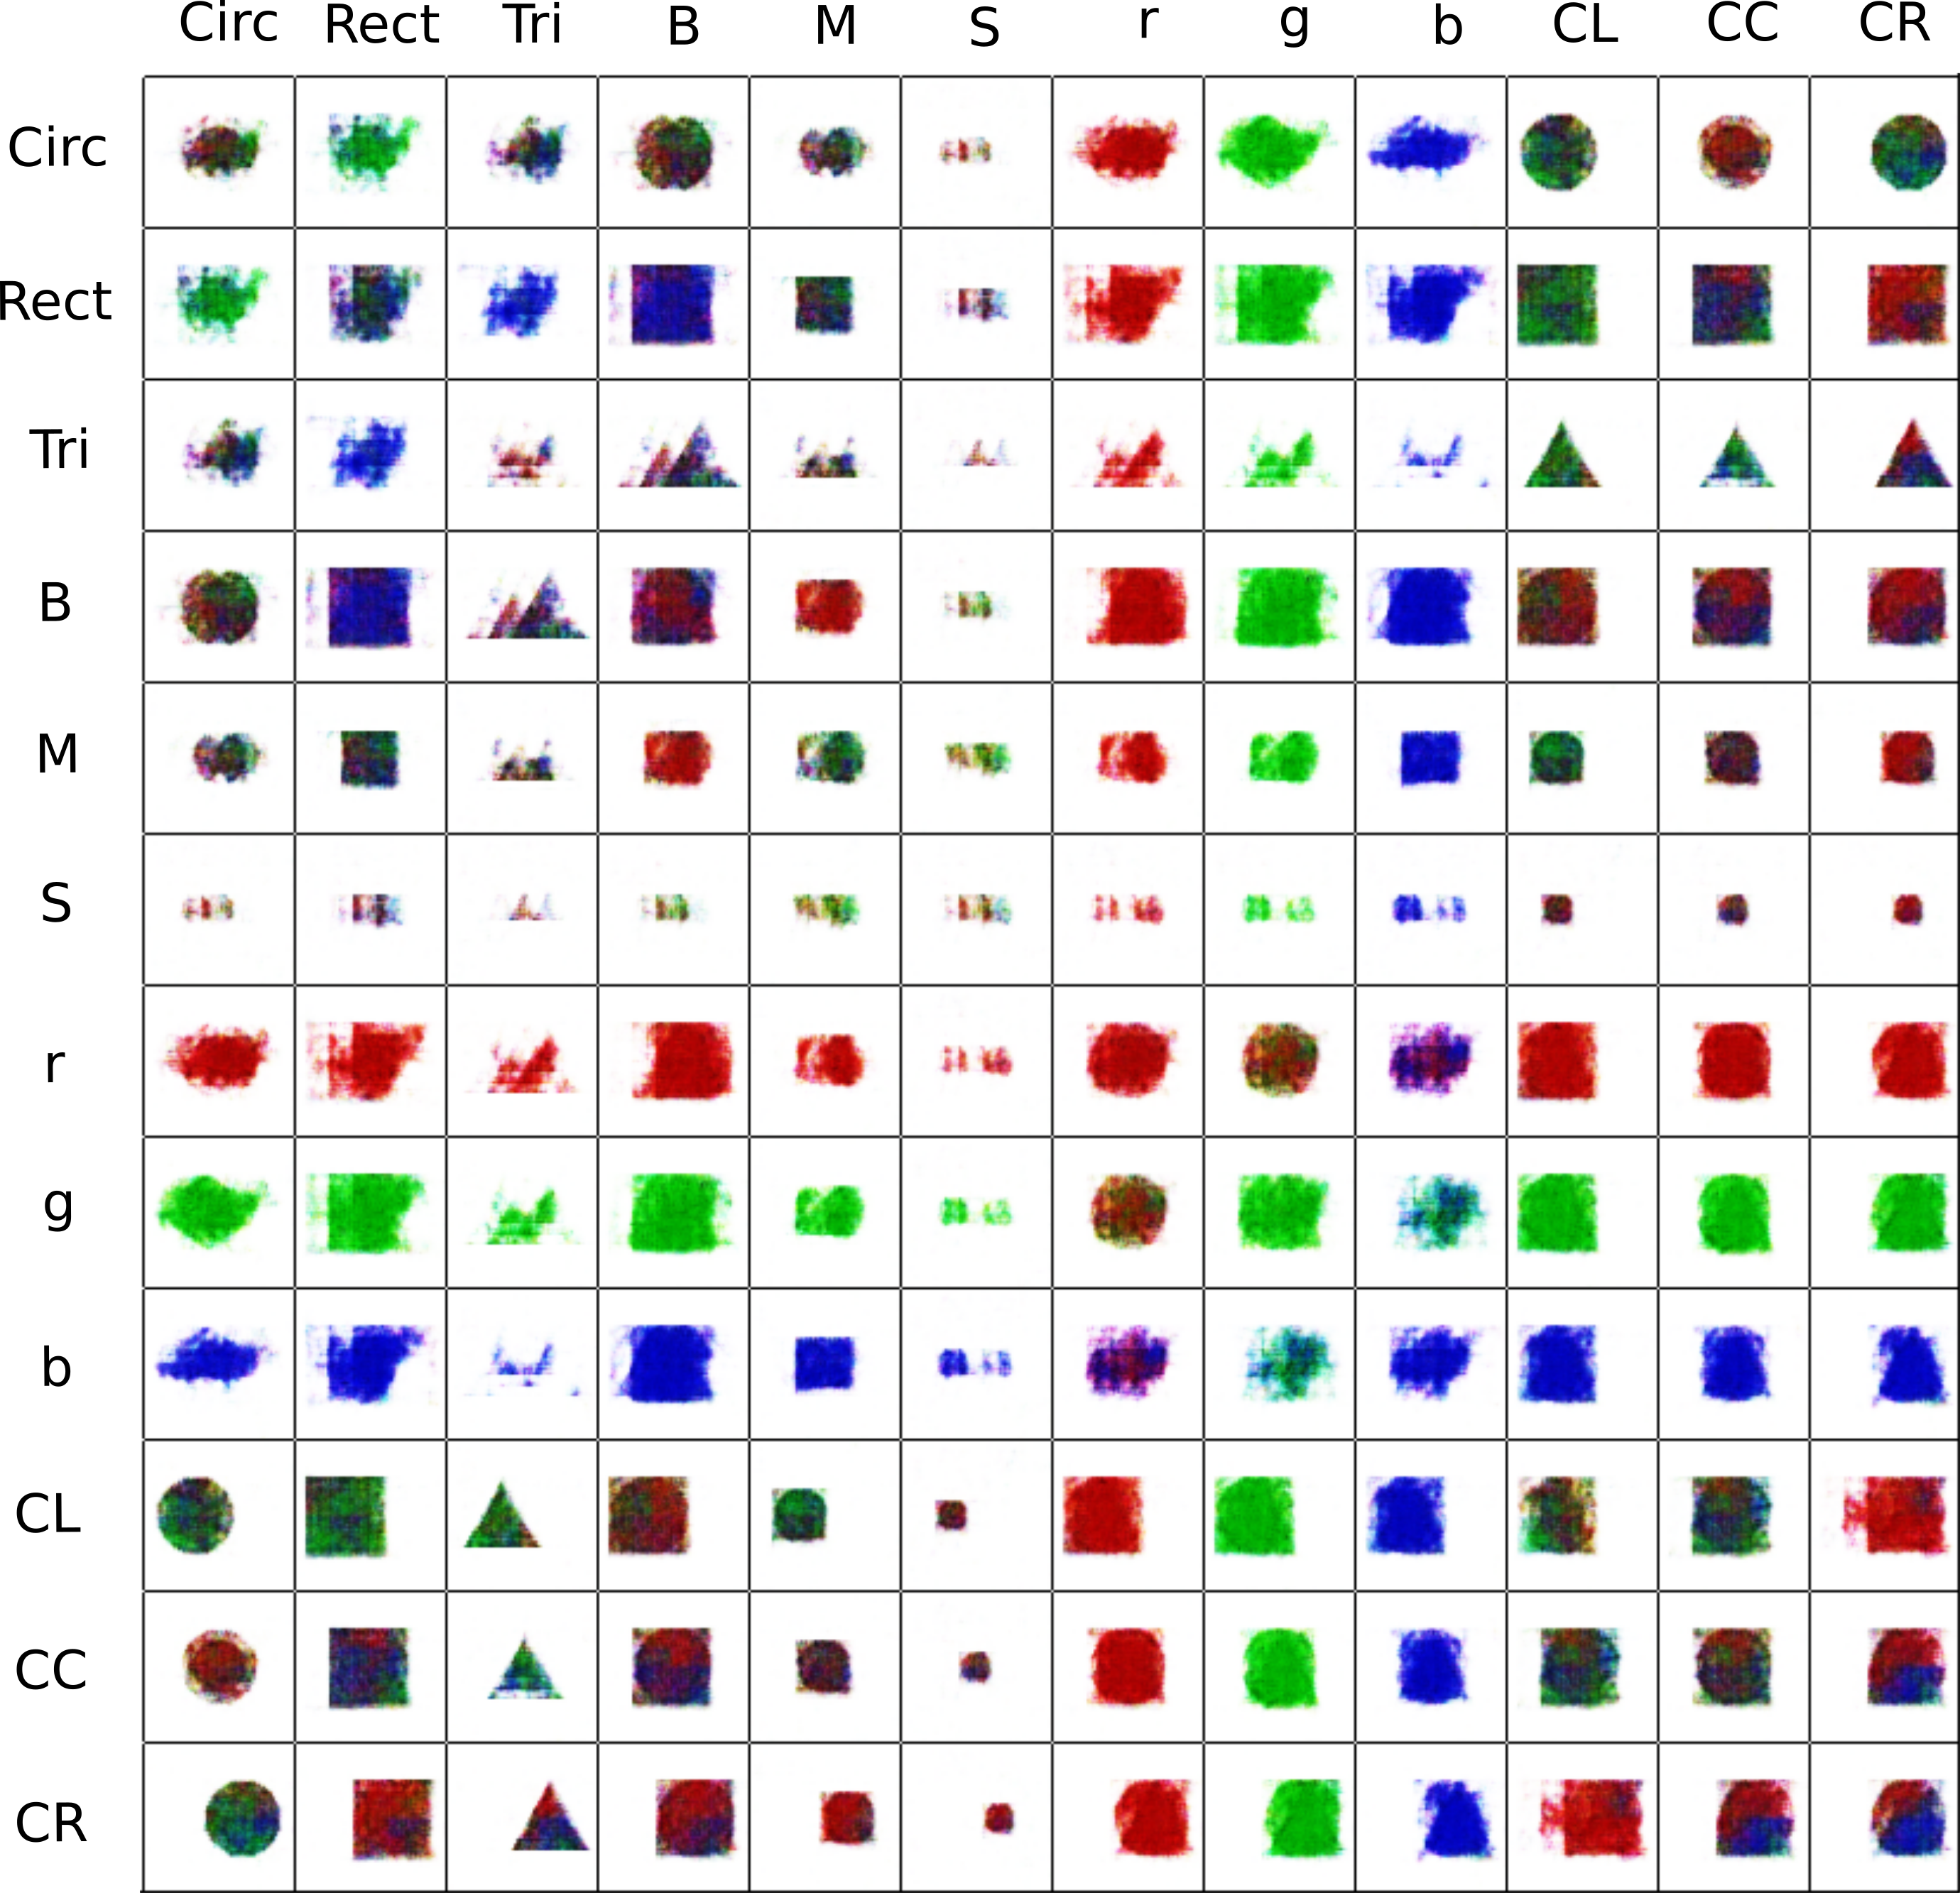
\includegraphics[width=0.75\textwidth]{Figs/shapes/2word333A.png}
%\caption{Images generated using word pairs using an embedding size of 296 neurons from experiment 2 run A.}
%\label{fig:2word333A}
%\end{figure}
%
%\begin{figure}
%\centering
%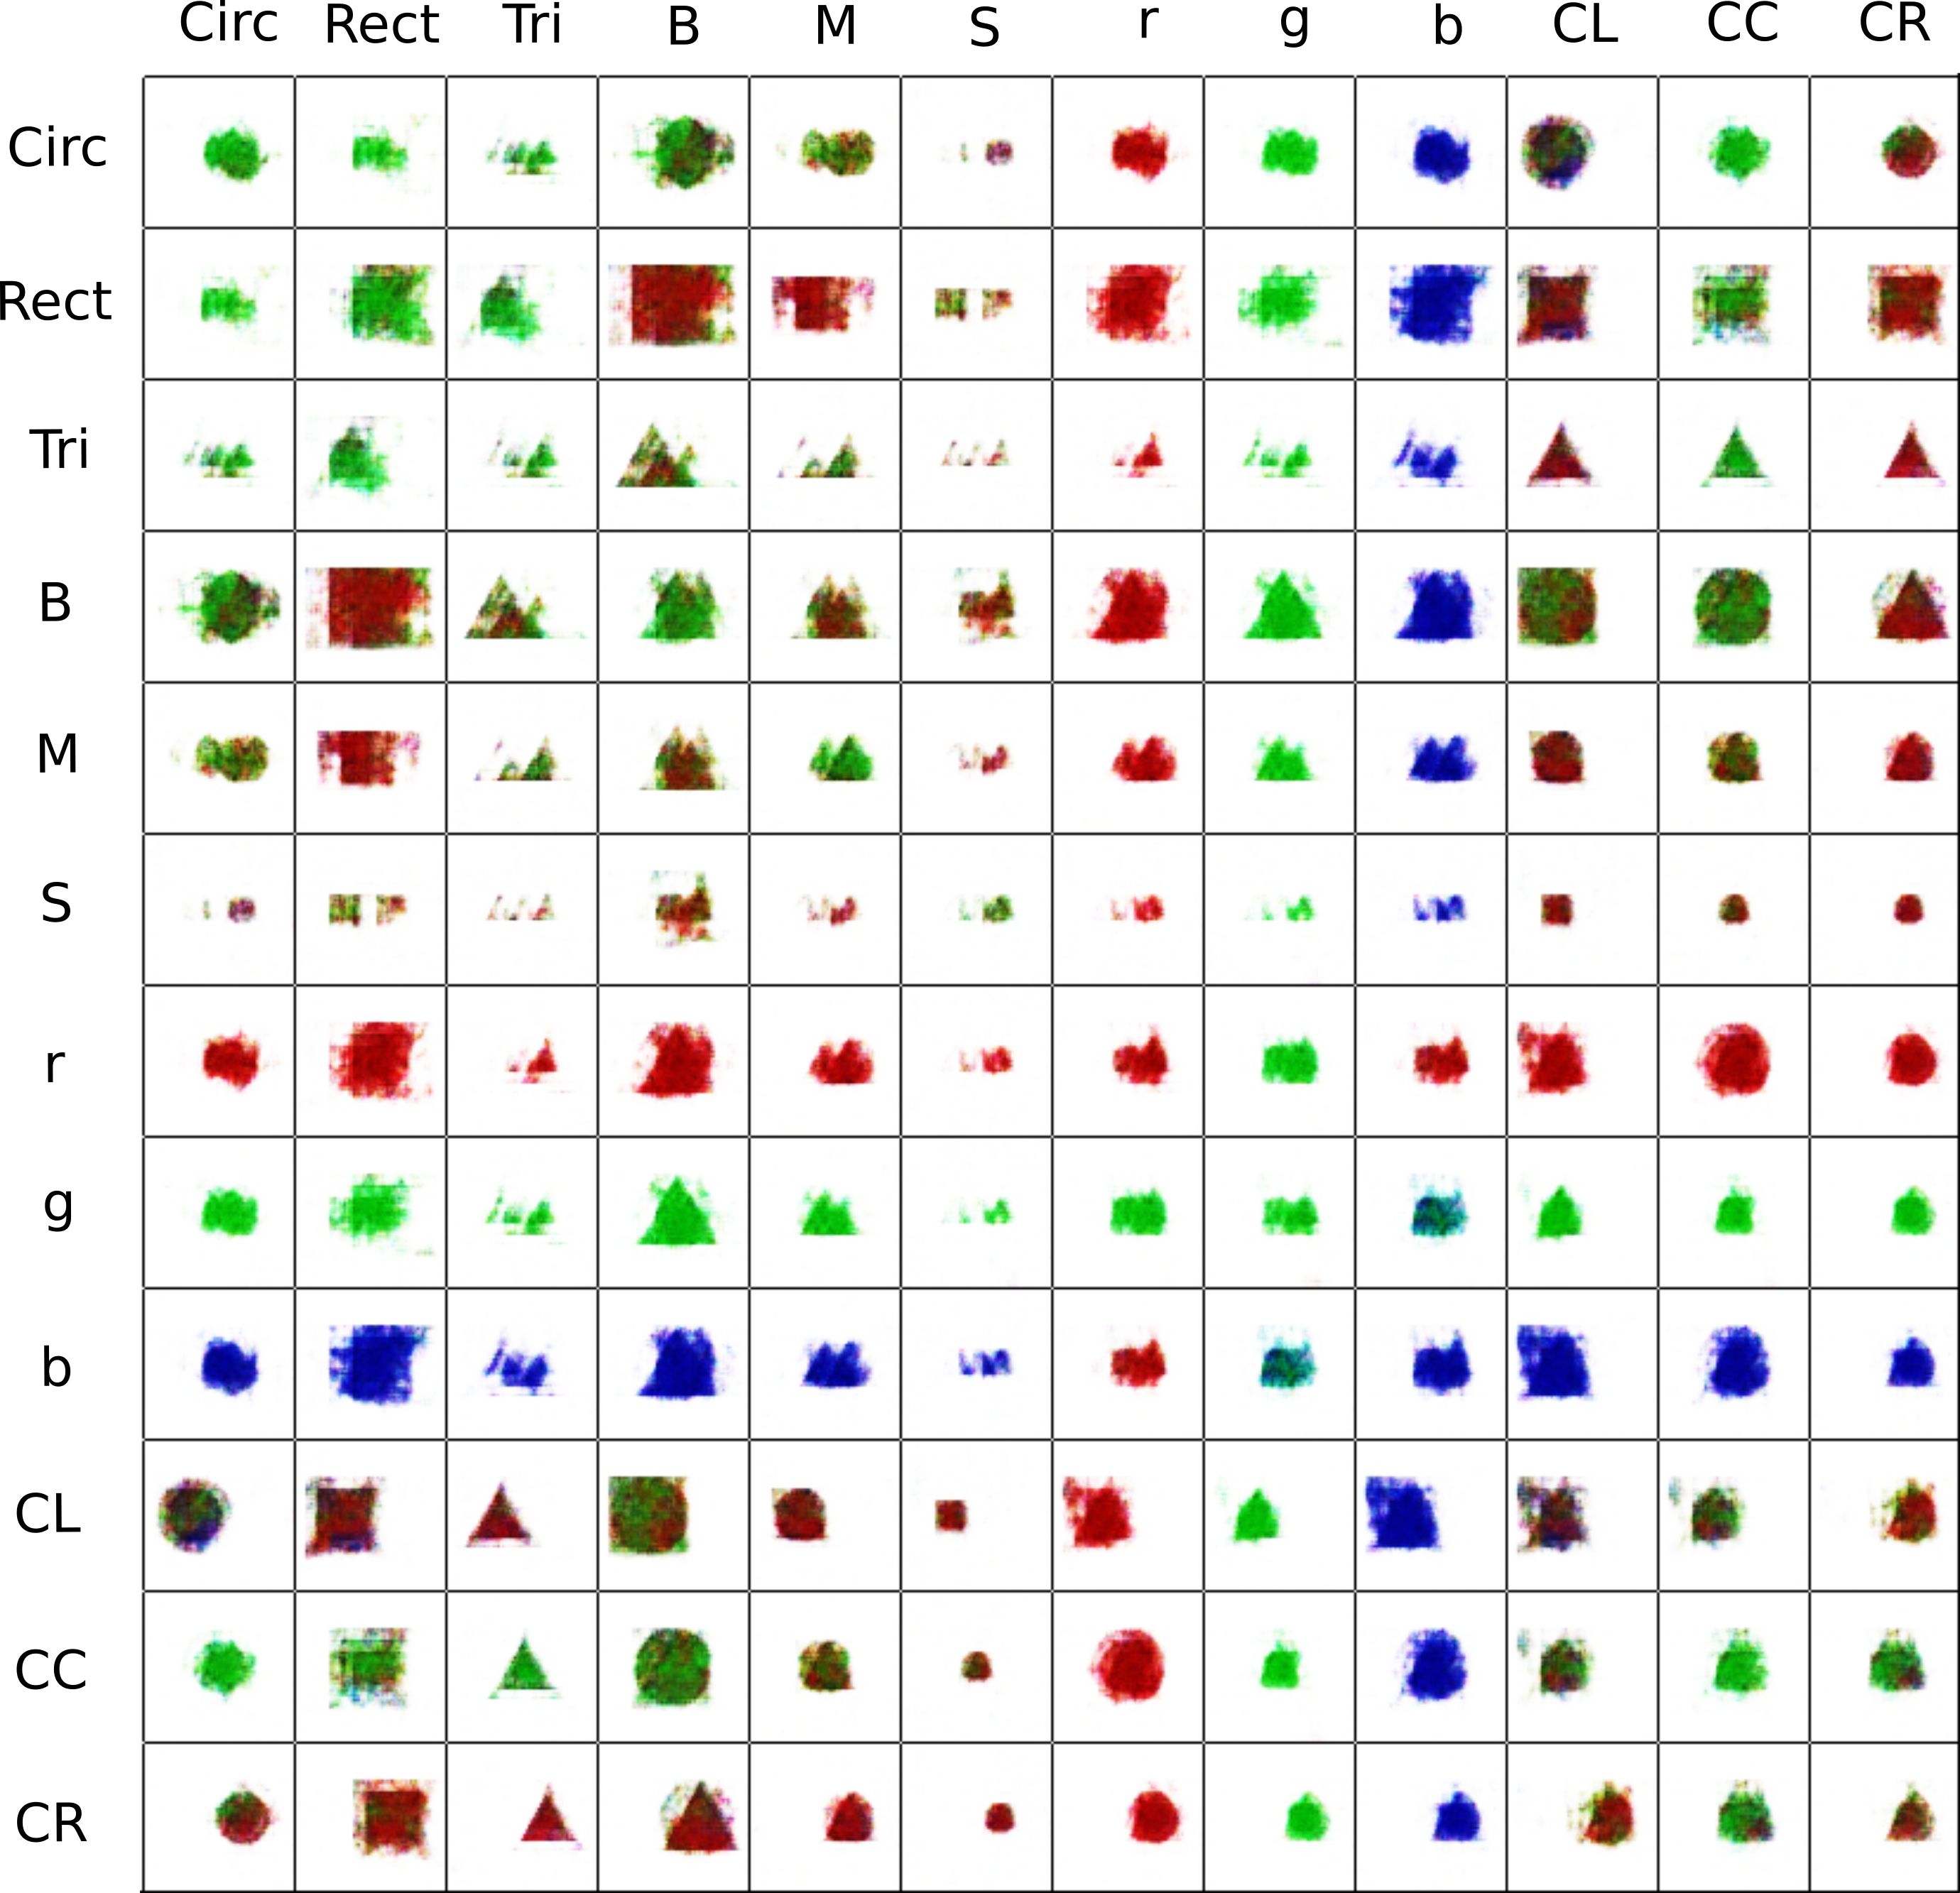
\includegraphics[width=0.75\textwidth]{Figs/shapes/2word333B.png}
%\caption{Images generated using word pairs using an embedding size of 296 neurons from experiment 2 run B.}
%\label{fig:2word333B}
%\end{figure}
%
%\begin{figure}
%\centering
%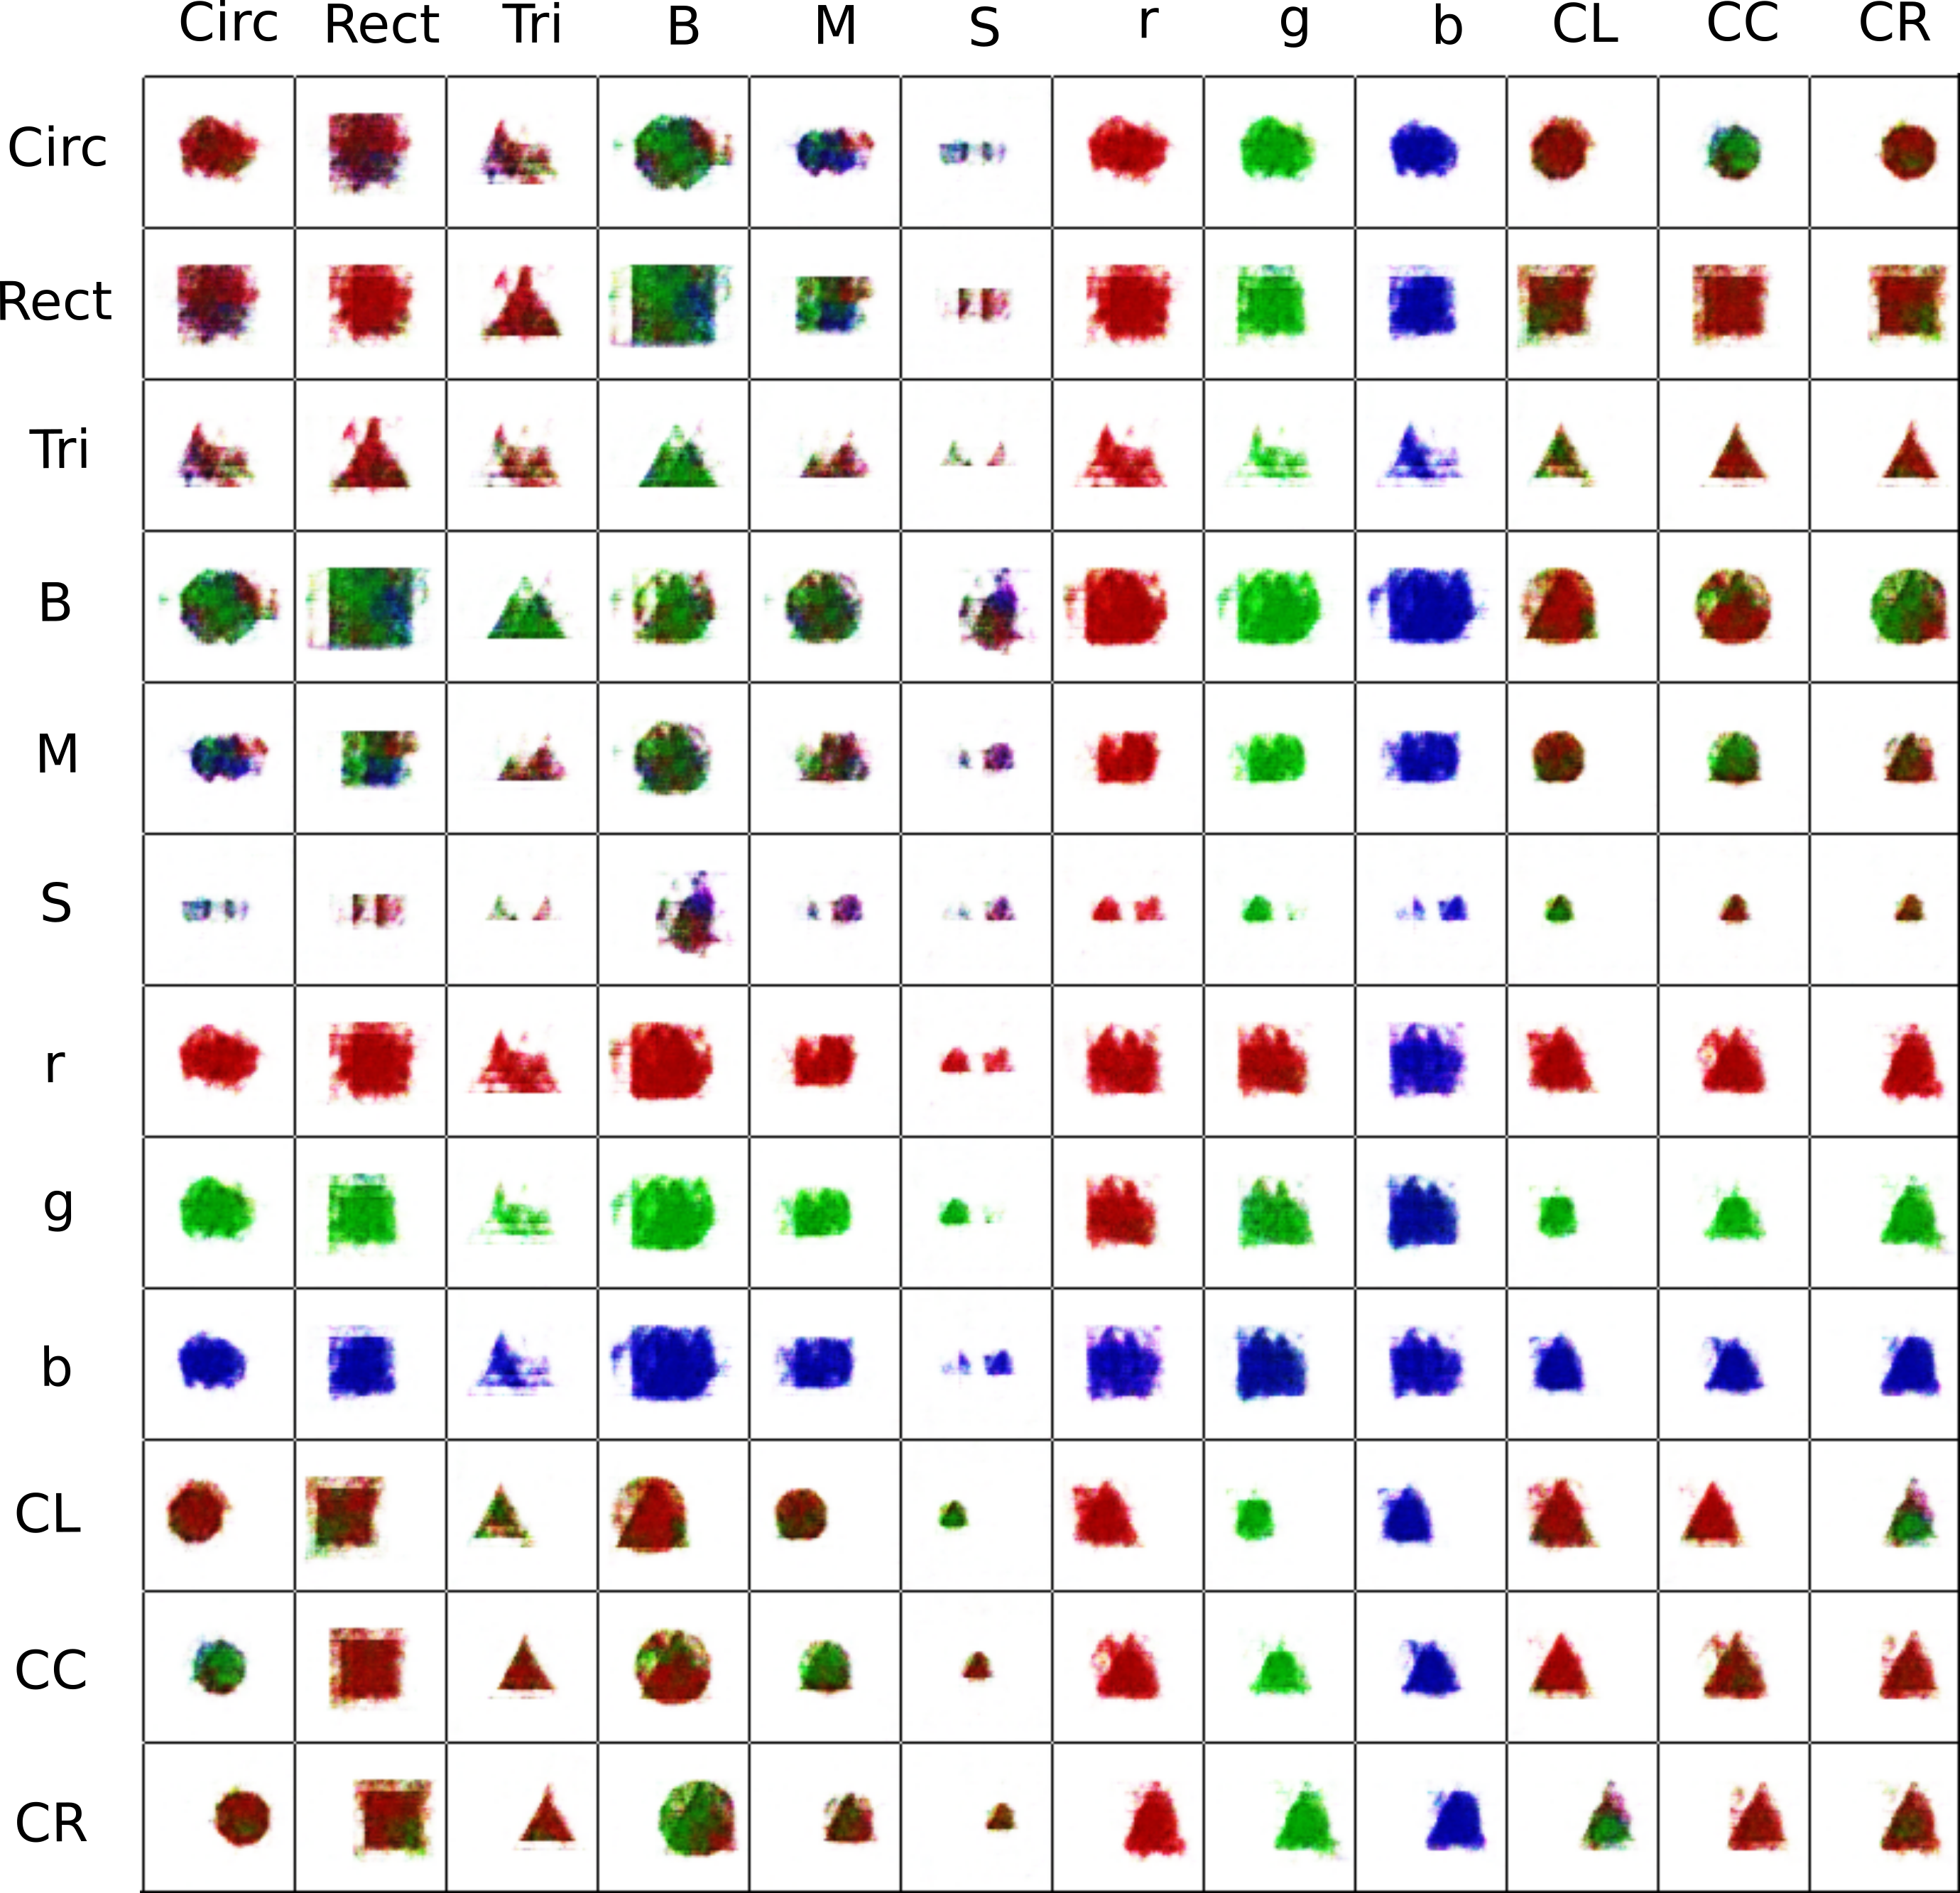
\includegraphics[width=0.75\textwidth]{Figs/shapes/2word333C.png}
%\caption{Images generated using word pairs using an embedding size of 296 neurons from experiment 2 run C.}
%\label{fig:2word333C}
%\end{figure}
%
%\begin{figure}
%\centering
%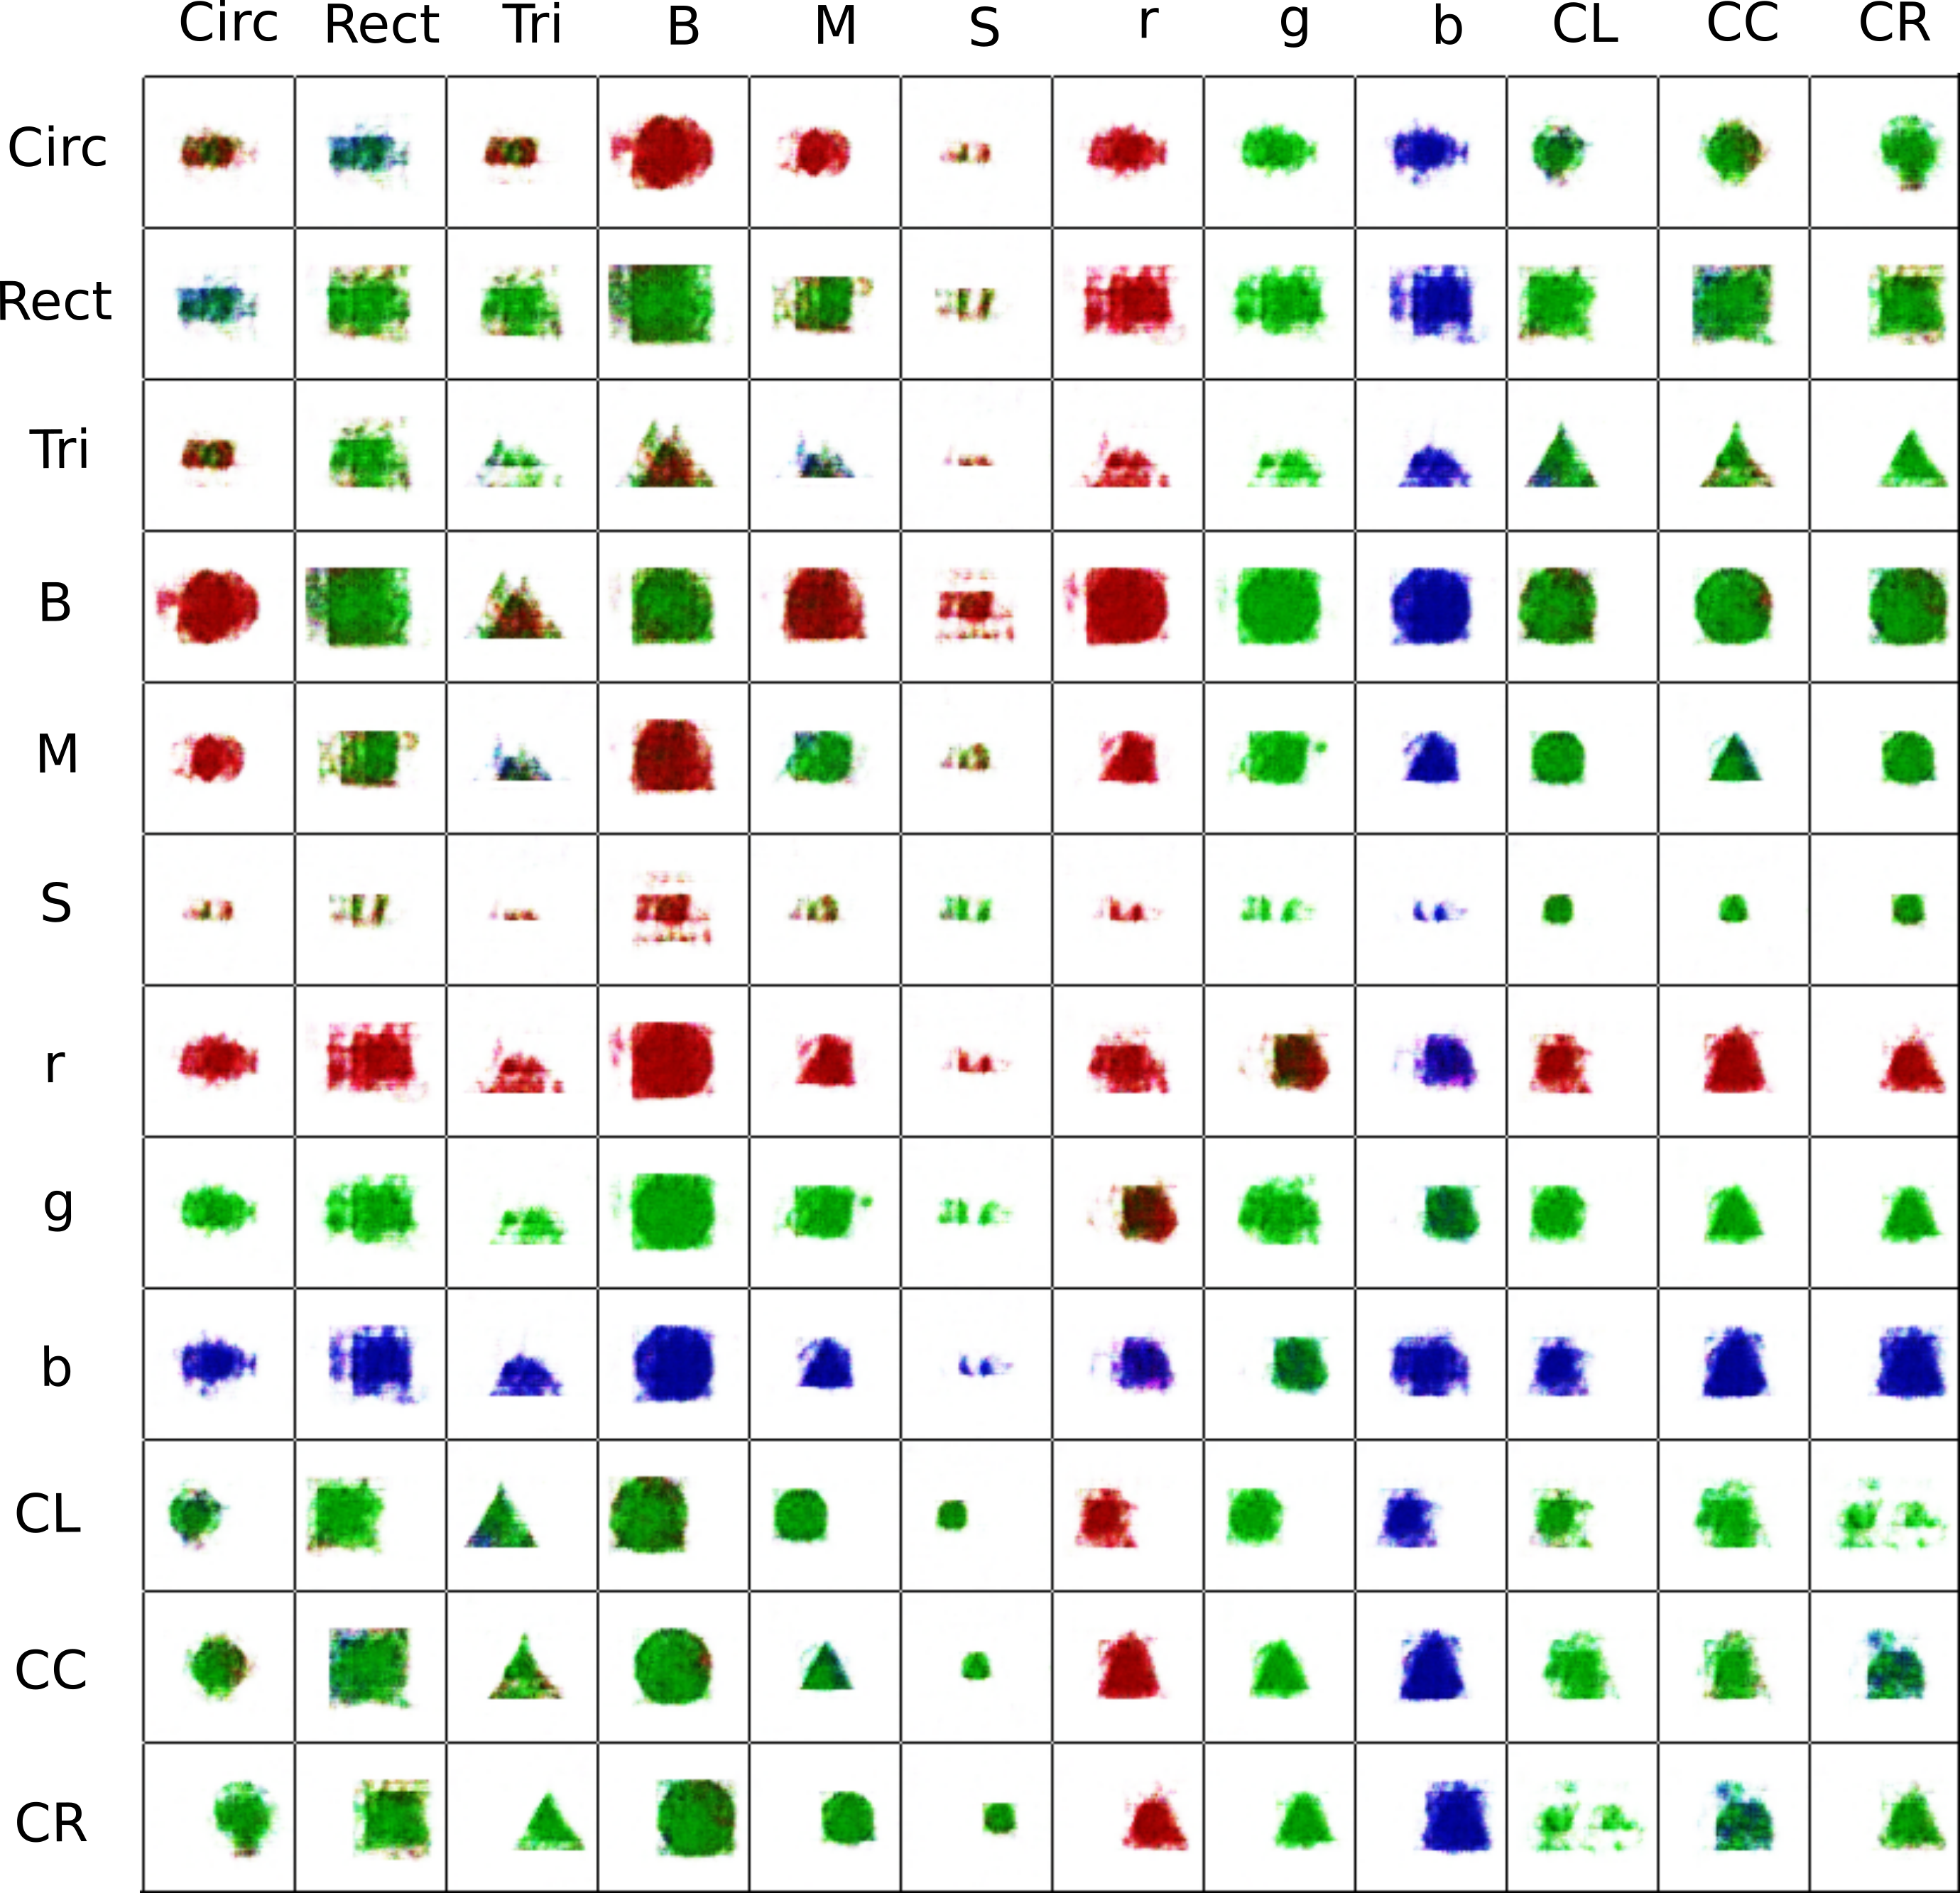
\includegraphics[width=0.75\textwidth]{Figs/shapes/2word333D.png}
%\caption{Images generated using word pairs using an embedding size of 296 neurons from experiment 2 run D.}
%\label{fig:2word333D}
%\end{figure}
%
%
%
%\begin{figure}
%\centering
%\includegraphics[width=\textwidth]{Figs/shapes/2word339A.png}
%\caption{Images generated using word pairs using a MAE initialised with random weights for experiment 3 run A.}
%\label{fig:2word339A}
%\end{figure}
%
%\begin{figure}
%\centering
%\includegraphics[width=\textwidth]{Figs/shapes/2word339B.png}
%\caption{Images generated using word pairs using a MAE initialised with random weights for experiment 3 run B.}
%\label{fig:2word339B}
%\end{figure}
%
%\begin{figure}
%\centering
%\includegraphics[width=\textwidth]{Figs/shapes/2word339C.png}
%\caption{Images generated using word pairs using a MAE initialised with random weights for experiment 3 run C.}
%\label{fig:2word339C}
%\end{figure}
%
%\begin{figure}
%\centering
%\includegraphics[width=\textwidth]{Figs/shapes/2word339D.png}
%\caption{Images generated using word pairs using a MAE initialised with random weights for experiment 3 run D.}
%\label{fig:2word339D}
%\end{figure}
%
%\begin{figure}
%\centering
%\includegraphics[width=\textwidth]{Figs/shapes/2word339A1.png}
%\caption{Images generated using word pairs using a MAE initialised with weights from experiment 1 for experiment 3 run A.}
%\label{fig:2word339A1}
%\end{figure}
%
%\begin{figure}
%\centering
%\includegraphics[width=\textwidth]{Figs/shapes/2word339B1.png}
%\caption{Images generated using word pairs using a MAE initialised with weights from experiment 1 forexperiment 3 run B.}
%\label{fig:2word339B1}
%\end{figure}
%
%\begin{figure}
%\centering
%\includegraphics[width=\textwidth]{Figs/shapes/2word339C1.png}
%\caption{Images generated using word pairs using a MAE initialised with weights from experiment 1 for experiment 3 run C.}
%\label{fig:2word339C1}
%\end{figure}
%
%\begin{figure}
%\centering
%\includegraphics[width=\textwidth]{Figs/shapes/2word339D1.png}
%\caption{Images generated using word pairs using a MAE initialised with weights from experiment 1 for experiment 3 run D.}
%\label{fig:2word339D1}
%\end{figure}
%
%\begin{figure}
%\centering
%\includegraphics[width=\textwidth]{Figs/shapes/2word339A2.png}
%\caption{Images generated using word pairs using a MAE initialised with weights from experiment 2 for experiment 3 run A.}
%\label{fig:2word339A2}
%\end{figure}
%
%\begin{figure}
%\centering
%\includegraphics[width=\textwidth]{Figs/shapes/2word339B2.png}
%\caption{Images generated using word pairs using a MAE initialised with weights from experiment 2 forexperiment 3 run B.}
%\label{fig:2word339B2}
%\end{figure}
%
%\begin{figure}
%\centering
%\includegraphics[width=\textwidth]{Figs/shapes/2word339C2.png}
%\caption{Images generated using word pairs using a MAE initialised with weights from experiment 2 for experiment 3 run C.}
%\label{fig:2word339C2}
%\end{figure}
%
%\begin{figure}
%\centering
%\includegraphics[width=\textwidth]{Figs/shapes/2word339D2.png}
%\caption{Images generated using word pairs using a MAE initialised with weights from experiment 2 for experiment 3 run D.}
%\label{fig:2word339D2}
%\end{figure}
%
%
%
%
%\begin{figure}
%\centering
%\includegraphics[width=\textwidth]{Figs/shapes/2word739A.png}
%\caption{Images generated using word pairs using a MAE initialised with random weights for experiment 4 run A.}
%\label{fig:2word739A}
%\end{figure}
%
%\begin{figure}
%\centering
%\includegraphics[width=\textwidth]{Figs/shapes/2word739B.png}
%\caption{Images generated using word pairs using a MAE initialised with random weights for experiment 4 run B.}
%\label{fig:2word739B}
%\end{figure}
%
%\begin{figure}
%\centering
%\includegraphics[width=\textwidth]{Figs/shapes/2word739C.png}
%\caption{Images generated using word pairs using a MAE initialised with random weights for experiment 4 run C.}
%\label{fig:2word739C}
%\end{figure}
%
%\begin{figure}
%\centering
%\includegraphics[width=\textwidth]{Figs/shapes/2word739D.png}
%\caption{Images generated using word pairs using a MAE initialised with random weights for experiment 4 run D.}
%\label{fig:2word739D}
%\end{figure}
%
%
%\begin{figure}
%\centering
%\includegraphics[width=\textwidth]{Figs/shapes/2word739A1.png}
%\caption{Images generated using word pairs using a MAE initialised with weights from experiment 1 for experiment 4 run A.}
%\label{fig:2word739A1}
%\end{figure}
%
%\begin{figure}
%\centering
%\includegraphics[width=\textwidth]{Figs/shapes/2word739B1.png}
%\caption{Images generated using word pairs using a MAE initialised with weights from experiment 1 for experiment 4 run B.}
%\label{fig:2word739B1}
%\end{figure}
%
%\begin{figure}
%\centering
%\includegraphics[width=\textwidth]{Figs/shapes/2word739C1.png}
%\caption{Images generated using word pairs using a MAE initialised with weights from experiment 1 for experiment 4 run C.}
%\label{fig:2word739C1}
%\end{figure}
%
%\begin{figure}
%\centering
%\includegraphics[width=\textwidth]{Figs/shapes/2word739D1.png}
%\caption{Images generated using word pairs using a MAE initialised with weights from experiment 1 for experiment 4 run D.}
%\label{fig:2word739D1}
%\end{figure}
%
%\begin{figure}
%\centering
%\includegraphics[width=\textwidth]{Figs/shapes/2word739A2.png}
%\caption{Images generated using word pairs using a MAE initialised with weights from experiment 2 for experiment 4 run A.}
%\label{fig:2word739A2}
%\end{figure}
%
%\begin{figure}
%\centering
%\includegraphics[width=\textwidth]{Figs/shapes/2word739B2.png}
%\caption{Images generated using word pairs using a MAE initialised with weights from experiment 2 for experiment 4 run B.}
%\label{fig:2word739B2}
%\end{figure}
%
%\begin{figure}
%\centering
%\includegraphics[width=\textwidth]{Figs/shapes/2word739C2.png}
%\caption{Images generated using word pairs using a MAE initialised with weights from experiment 2 for experiment 4 run C.}
%\label{fig:2word739C2}
%\end{figure}
%
%\begin{figure}
%\centering
%\includegraphics[width=\textwidth]{Figs/shapes/2word739D2.png}
%\caption{Images generated using word pairs using a MAE initialised with weights from experiment 2 for experiment 4 run D.}
%\label{fig:2word739D2}
%\end{figure}
%
%
%\begin{figure}
%\centering
%\includegraphics[width=\textwidth]{Figs/shapes/2word739A3.png}
%\caption{Images generated using word pairs using a MAE initialised with weights from experiment 3 for experiment 4 run A.}
%\label{fig:2word739A3}
%\end{figure}
%
%\begin{figure}
%\centering
%\includegraphics[width=\textwidth]{Figs/shapes/2word739B3.png}
%\caption{Images generated using word pairs using a MAE initialised with weights from experiment 3 for experiment 4 run B.}
%\label{fig:2word739B3}
%\end{figure}
%
%\begin{figure}
%\centering
%\includegraphics[width=\textwidth]{Figs/shapes/2word739C3.png}
%\caption{Images generated using word pairs using a MAE initialised with weights from experiment 3 for experiment 4 run C.}
%\label{fig:2word739C3}
%\end{figure}
%
%\begin{figure}
%\centering
%\includegraphics[width=\textwidth]{Figs/shapes/2word739D3.png}
%\caption{Images generated using word pairs using a MAE initialised with weights from experiment 3 for experiment 4 run D.}
%\label{fig:2word739D3}
%\end{figure}
%
%
%\begin{figure}
%\centering
%\includegraphics[width=\textwidth]{Figs/shapes/2word739A31.png}
%\caption{Images generated using word pairs using a MAE initialised with weights from experiment 1 + 3 for experiment 4 run A.}
%\label{fig:2word739A31}
%\end{figure}
%
%\begin{figure}
%\centering
%\includegraphics[width=\textwidth]{Figs/shapes/2word739B31.png}
%\caption{Images generated using word pairs using a MAE initialised with weights from experiment 1 + 3 for experiment 4 run B.}
%\label{fig:2word739B31}
%\end{figure}
%
%\begin{figure}
%\centering
%\includegraphics[width=\textwidth]{Figs/shapes/2word739C31.png}
%\caption{Images generated using word pairs using a MAE initialised with weights from experiment 1 + 3 for experiment 4 run C.}
%\label{fig:2word739C31}
%\end{figure}
%
%\begin{figure}
%\centering
%\includegraphics[width=\textwidth]{Figs/shapes/2word739D31.png}
%\caption{Images generated using word pairs using a MAE initialised with weights from experiment 1 for experiment 4 run D.}
%\label{fig:2word739D31}
%\end{figure}
%
%
%
%
%
%\begin{figure}
%\centering
%\includegraphics[width=\textwidth]{Figs/shapes/2word739A32.png}
%\caption{Images generated using word pairs using a MAE initialised with weights from experiment 2 + 3 for experiment 4 run A.}
%\label{fig:2word739A32}
%\end{figure}
%
%\begin{figure}
%\centering
%\includegraphics[width=\textwidth]{Figs/shapes/2word739B32.png}
%\caption{Images generated using word pairs using a MAE initialised with weights from experiment 2 + 3 for experiment 4 run B.}
%\label{fig:2word739B32}
%\end{figure}
%
%\begin{figure}
%\centering
%\includegraphics[width=\textwidth]{Figs/shapes/2word739C32.png}
%\caption{Images generated using word pairs using a MAE initialised with weights from experiment 2 + 3 for experiment 4 run C.}
%\label{fig:2word739C32}
%\end{figure}
%
%\begin{figure}
%\centering
%\includegraphics[width=\textwidth]{Figs/shapes/2word739D32.png}
%\caption{Images generated using word pairs using a MAE initialised with weights from experiment 2 for experiment 4 run D.}
%\label{fig:2word739D32}
%\end{figure}



